% Autor: Leonhard Segger, Alexander Neuwirth
% Datum: 2017-10-30
\documentclass[
	% Papierformat
	a4paper,
	% Schriftgröße (beliebige Größen mit „fontsize=Xpt“)
	12pt,
	% Schreibt die Papiergröße korrekt ins Ausgabedokument
	pagesize,
	% Sprache für z.B. Babel
	ngerman
]{scrartcl}

% Achtung: Die Reihenfolge der Pakete kann (leider) wichtig sein!
% Insbesondere sollten (so wie hier) babel, fontenc und inputenc (in dieser
% Reihenfolge) als Erstes und hyperref und cleveref (Reihenfolge auch hier
% beachten) als Letztes geladen werden!

\usepackage{tikz}
\usetikzlibrary{calc,patterns,angles,quotes} % loads some tikz extensions\usepackage{tikz}
\usetikzlibrary{babel}

% Silbentrennung etc.; Sprache wird durch Option bei \documentclass festgelegt
\usepackage{babel}
% Verwendung der Zeichentabelle T1 (Sonderzeichen etc.)
\usepackage[T1]{fontenc}
% Legt die Zeichenkodierung der Eingabedatei fest, z.B. UTF-8
\usepackage[utf8]{inputenc}
% Schriftart
\usepackage{lmodern}
% Zusätzliche Sonderzeichen
\usepackage{textcomp}

% Mathepaket (intlimits: Grenzen über/unter Integralzeichen)
\usepackage[intlimits]{amsmath}
% Ermöglicht die Nutzung von \SI{Zahl}{Einheit} u.a.
\usepackage{siunitx}
% Zum flexiblen Einbinden von Grafiken (\includegraphics)
\usepackage{graphicx}
% Abbildungen im Fließtext
\usepackage{wrapfig}
% Abbildungen nebeneinander (subfigure, subtable)
\usepackage{subcaption}
% Funktionen für Anführungszeichen
\usepackage{csquotes}
\MakeOuterQuote{"}
% Zitieren, Bibliografie
\usepackage[sorting=none]{biblatex}


% Zur Darstellung von Webadressen
\usepackage{url}
%chemische Formeln
\usepackage[version=4]{mhchem}
% siunitx: Deutsche Ausgabe, Messfehler getrennt mit ± ausgeben
\usepackage{floatrow}
\floatsetup[table]{capposition=top}
\usepackage{float}
% Verlinkt Textstellen im PDF-Dokument
\usepackage[unicode]{hyperref}
% "Schlaue" Referenzen (nach hyperref laden!)
\usepackage{cleveref}
\sisetup{
	locale=DE,
	separate-uncertainty
}
\bibliography{BA-C-04_AFM_05-11-2018_References}

\begin{document}

	\begin{titlepage}
		\centering
		{\scshape\LARGE Versuchsbericht zu \par}
		\vspace{1cm}
		{\scshape\huge AFM - Raster-Kraft-Mikroskopie \par}
		\vspace{2.5cm}
		{\LARGE Gruppe BA-C-04 \par}
		\vspace{0.5cm}

		{\large Alexander Neuwirth (E-Mail: a\_neuw01@wwu.de) \par}
		{\large Leonhard Segger (E-Mail: l\_segg03@uni-muenster.de) \par}
		\vfill

		durchgeführt am 05.11.18\par
		betreut von\par
		{\large Anne Bakker}

		\vfill

		{\large \today\par}
	\end{titlepage}
	\tableofcontents
	\newpage

	%TODO Raster-Kraft-Mikroskop bzw. Rasterkraftmikroskop: sollte  maybe einheitlich sein, ich stimme für ohne Bindestriche, weil das sagt Wikipedia und die Anleitung, aber der Titel ist halt mit Bindestrichen

	\section{Kurzfassung}
	% Hypothese	und deren Ergebnis, wenn Hypothese ist, dass nur Theorie erfüllt, sagen: Erwartung: Theorie aus einführung (mit reflink) erfüllt
	% Ergebnisse, auch Zahlen, mindestens wenn's halbwegs Sinn ergibt
	% Was wurde gemacht
	% manche leute wollen Passiv oder "man", manche nicht
	Die Raster-Kraft-Mikroskopie (AFM von engl. atomic force microscopy) ist ein Verfahren, welches es erlaubt mit optisch nicht erreichbarer Auflösung Oberflächenprofile zu erstellen sowie Kräfte zwischen Probenoberfläche und Messspitze zu bestimmen.
	Es werden im Wesentlichen drei Untersuchungen durchgeführt.
	Zunächst wird im Kontaktmodus die Oberflächenstruktur von drei Proben bestimmt, anhand derer diese den optischen Speichertechnologien CD, DVD und Blu-ray Disc zugeordnet werden.
	Diese Zuordnung kann mit hoher Gewissheit vorgenommen werden.
	Dann wird durch Kraft-Distanz-Spektroskopie die Adhäsion als Gemisch der auftretenden Kräfte zwischen Spitze und den Proben untersucht.
	Zuletzt wird mithilfe einer Probe aus sehr dünnen Spitzen die Topografie der Cantilever-Spitze untersucht.
	Das Ergebnis dessen kann nicht mit den Herstellerangaben in Einklang gebracht werden.
	Es werden außerdem Möglichkeiten der erweiterten Untersuchung diskutiert.

	\section{Theorie}
	\label{sec_theorie}

	\subsection{Allgemeines}
	Ein Raster-Kraft-Mikroskop fährt eine Spitze an einem flexiblen Balken (Cantilever) rasterförmig über die Probenoberfläche, um ein Oberflächenprofil zu erstellen.

	Das gemessene Profil ist nicht nur von der Topografie der Probe, sondern auch der der Spitze abhängig.
	Wenn der Spitzenradius gegenüber den betrachteten Strukturen klein ist, kann man die Oberflächenstruktur der Proben messen.
	Ist es jedoch umgekehrt, dominiert die Spitzentopografie die Messung, was genutzt werden kann, um den Spitzenradius zu bestimmen.

	In \cref{fig_Aufbau} ist die Funktionsweise des AFMs skizziert, welche im Folgenden erläutert werden soll.
	Es ist zwischen statischem und dynamischem Modus zu unterscheiden.



	\subsection{Statischer Modus (Kontaktmodus)}
	Im statischem Modus wird die Spitze des Cantilevers in Kontakt mit der Probe gebracht.
	Dann wird die Spitze in einem Raster über die Probe gefahren, wofür sie durch Piezokristalle bewegt wird.
	Diese haben eine von der an sie angelegten Spannung abhängige Ausdehnung.
	Dieser Zusammenhang ist nicht bekannt und muss wie in \cref{sec_methoden} durch eine Kalibrierprobe bestimmt werden.
	Es wird die Spitze mit einer bestimmten Kraft (Normalkraft) auf die Probe gedrückt, die nach dem Hookeschen Gesetz einer bestimmten Verbiegung des Cantilevers entspricht.
	Letztere wird durch einen Laser gemessen, der vom Cantilever  reflektiert wird, weshalb seine Position auf einer Photodiode abhängig von der Verbiegung des Cantilevers ist. %hier steht viel "Verbiegung des Cantilevers"... % 'seine'=Laser, aber kann halt vieles sein
	Die Verbiegung des Cantilevers wird durch eine Regelung möglichst konstant gehalten, sodass die Abweichung zwischen auf den Cantilever ausgewirkten Kraft und der Normalkraft abhängig von der z-Position der Spitze ist.

	\begin{figure}[H]
		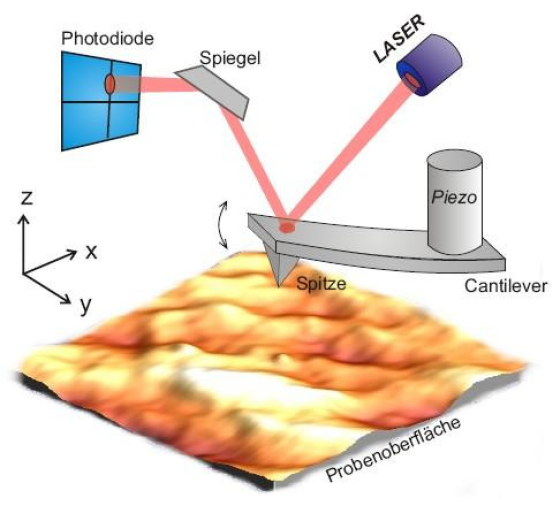
\includegraphics[width=0.5\textwidth]{images/sonstiges/Aufbau}
		\centering
		\caption{Schematischer Aufbau eines Raster-Kraft-Mikroskops. \cite{Anleitung}}
		\label{fig_Aufbau}
		\centering
	\end{figure}

	\subsection{Kraft-Abstands-Spektroskopie}
	Bei der Kraft-Abstands-Spektroskopie wird die Spitze langsam an die Probe angenähert.
	Die Rückstellkraft des Cantilevers wirkt hierbei den Anziehungskräften zwischen Probe und Spitze entgegen.
	In \cref{fig_KDS} ist der Verlauf der Kraft-Distanz-Kurve idealisiert dargestellt.
	An dem Abstand, an dem die Anziehungskräfte größer als die Rückstellkraft werden, springt die Spitze in Kontakt mit der Probe.
	Dieser Vorgang wird als \enquote{snap-in} bezeichnet.
	Eine weitere Annäherung führt zu einer Verbiegung des Cantilevers gemäß des Hookeschen Gesetzes.

	Bei Rückziehen der Spitze kommt es in analoger Art und Weise zu einem Punkt, an dem die Adhäsion genauso groß wie die Rückstellkraft des Cantilevers ist und es kommt zu einem \enquote{snap-off}.
	Demnach lässt sich aus dem Minimum der Kurve beim Zurückziehen die Adhäsionskraft zwischen Probe und Spitze bestimmen.

	\begin{figure}[H]
		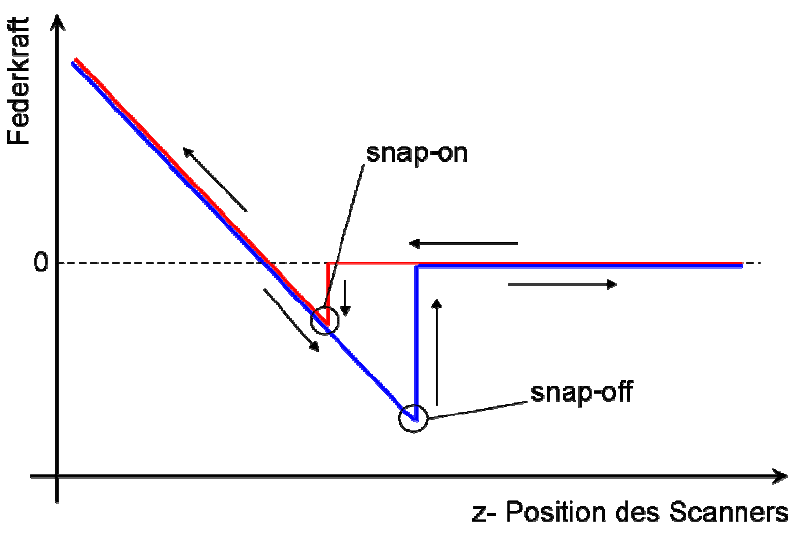
\includegraphics[width=0.7\textwidth]{images/sonstiges/KDS}
		\centering
		\caption{Schematischer Verlauf einer typischen Kraft-Distanz-Kurve im Kontakt-Modus. Die rote Kurve stellt den Verlauf bei der Annäherung, die blaue Kurve den Verlauf beim Zurückziehen der Spitze dar. Die auf der senkrechten Achse angegebene Federkraft wird bei den Messungen in diesem Versuchsprotokoll durch Auslenkung ersetzt, da das verwendete Programm dies gemäß des Hookeschen Gesetzes umrechnet. \cite{Anleitung}}
		\label{fig_KDS}
		\centering
	\end{figure}

	\subsection{Dynamischer Modus}
	Im dynamischen Modus befindet sich die Messspitze nicht in Kontakt mit der Probe, sondern schwingt über der Probenoberfläche.
	Dabei wird eine Anregungsfrequenz verwendet, die nahe an, aber nicht auf der Resonanzfrequenz liegt.
	Da die Kräfte zwischen Probe und Cantilever die effektive Rückstellkraft verändern, ändert sich die Resonanzfrequenz in Abhängigkeit vom Probe-Spitze-Abstand (bei anziehenden Kräften wird sie reduziert).
	Abhängig davon, ob dieser Abstand steigt oder sinkt, nähert sich die Resonanzfrequenz also der Anregungsfrequenz an oder entfernt sich von ihr.
	Eine Vergrößerung der Differenzfrequenz sorgt für eine verringerte Amplitude und umgekehrt.
	Die Messung der Amplitude der Schwingung erlaubt somit den Rückschluss auf das Oberflächenprofil, ohne dabei Spitze oder Probe mechanischen Abnutzungen auszusetzen.

	\section{Methoden}
	%TODO Bild crop, weil kleiner dann?
	\label{sec_methoden}
	In \cref{fig_Foto} ist das verwendete Mikroskop abgebildet.
	\begin{figure}[H]
		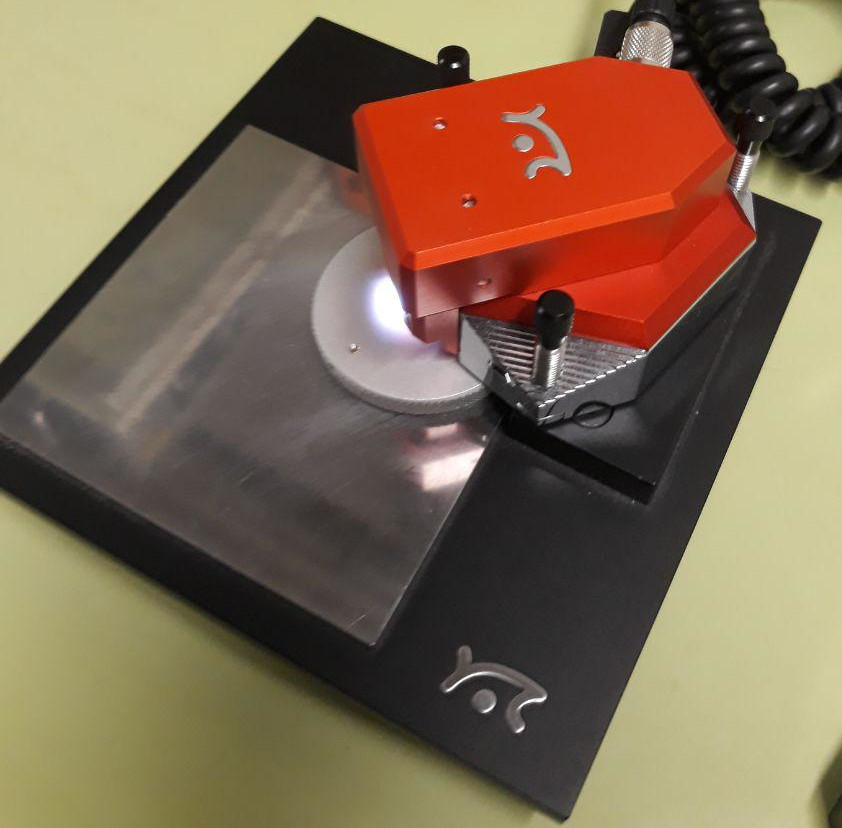
\includegraphics[width=0.5\textwidth]{images/afm}
		\centering
		\caption{Fotografie des verwendeten Raster-Kraft-Mikroskops.}
		\label{fig_Foto}
		\centering
	\end{figure}

	Es sind drei Proben gegeben, die Teil einer CD, DVD und Blu-ray Disc waren.
	Um zu bestimmen, welche Probe von welchem optischen Speichermedium stammt, wird die Raster-Kraft-Mikroskopie verwendet.
	Außerdem soll aus Kraft-Distanz-Kurven die Adhäsion der verschiedenen Oberflächen bestimmt werden und zuletzt der Radius einer Cantilever-Spitze untersucht werden.

	Zunächst wird die Oberflächenstruktur einer Kalibrierprobe im Kontaktmodus (Spitze: PPP-CONTR-50) untersucht, um den korrekten Zusammenhang zwischen Spannung an den Piezokristallen und Position der Cantilever-Spitze festzustellen.
	Der tatsächliche Wert dieses Zusammenhangs wird hier nicht bestimmt, da das Programm zur Ansteuerung des Raster-Kraft-Mikroskop bereits einen Zusammenhang annimmt und dieser durch die Kalibrierung lediglich korrigiert wird.
	Die Kalibrierprobe besteht dabei aus einer glatten Oberfläche, auf der Quader mit bekannter Höhe und quadratischer Grundfläche bekannter Seitenlänge aufgebracht sind.
	Die Kalibrierung wird in x-,y- und z-Richtung getrennt durchgeführt.

	Dann werden fünf Kraft-Distanz-Kurven an verschiedenen Stellen der Oberfläche der Quader aufgenommen.
	Diese erlauben wie in \cref{sec_theorie} beschrieben ein Maß für die Adhäsion der Oberfläche zu finden.

	Danach werden AFM-Aufnahmen der drei zuzuordnenden Proben gemacht, aus denen gemäß der Kalibrierung Pit-Länge, -Breite und -Tiefe bestimmt werden.
	Es ist anzumerken, dass zwei der Proben die Grundfläche des Speichermediums darstellen, sodass bei ihnen Pits Täler sind, während eine Probe die Schutzbeschichtung darstellt, weshalb hier die Pits als Berge auftreten.
	Aus der Bestimmung des Spurabstands lassen sich die Proben dann mithilfe von Referenzwerten den drei optischen Speichertechnologien zuordnen.

	Zuletzt wird der dynamische Modus (Spitze: PPP-NCLR-50) gewählt.
	Hierbei wird zunächst ein Resonanzprofil des Cantilevers aufgenommen und ein Wert auf der linken Flanke als Anregungsfrequenz verwendet.
	Dies maximiert die Empfindlichkeit, während Entfernung und Annäherung der Resonanzfrequenz unterscheidbar bleiben.
	Es wird eine Probe untersucht, deren Oberfläche aus Spitzen besteht, die als deutlich dünner als die Cantilever-Spitze angenommen werden.
	Dies erlaubt es den Radius der verwendeten Cantilever-Spitze abzuschätzen.
	Dafür wurden zunächst P-,I- und D-Anteil des PID-Reglers, der den Abstand zwischen Probe und Spitze konstant hält, auf ein möglichst störungsfreies, gleichmäßiges Bild optimiert.


	\section{Ergebnisse und Diskussion}


	\subsection{Beobachtung und Datenanalyse}

	Zunächst wird mit der Kamera eine Position geringer Verunreinigung auf dem Material gesucht.
	Wenn dennoch Unreinheiten gemessen werden, wird eine anderen Stelle untersucht.
	Die gemessenen Topografien weisen einen Höhengradienten auf und häufig fällt die gemessene Höhe nach einem Maximum nicht mehr auf Null zurück.
	Diese systematischen Fehler können mit dem Programm "Gwyddion" behoben werden (vgl. \cref{fig_kali_raw} mit \cref{fig_kali_top}).
	Außerdem wird die z-Achse so verschoben, dass das globale Minimum auf Null liegt.

	\begin{figure}[H]
			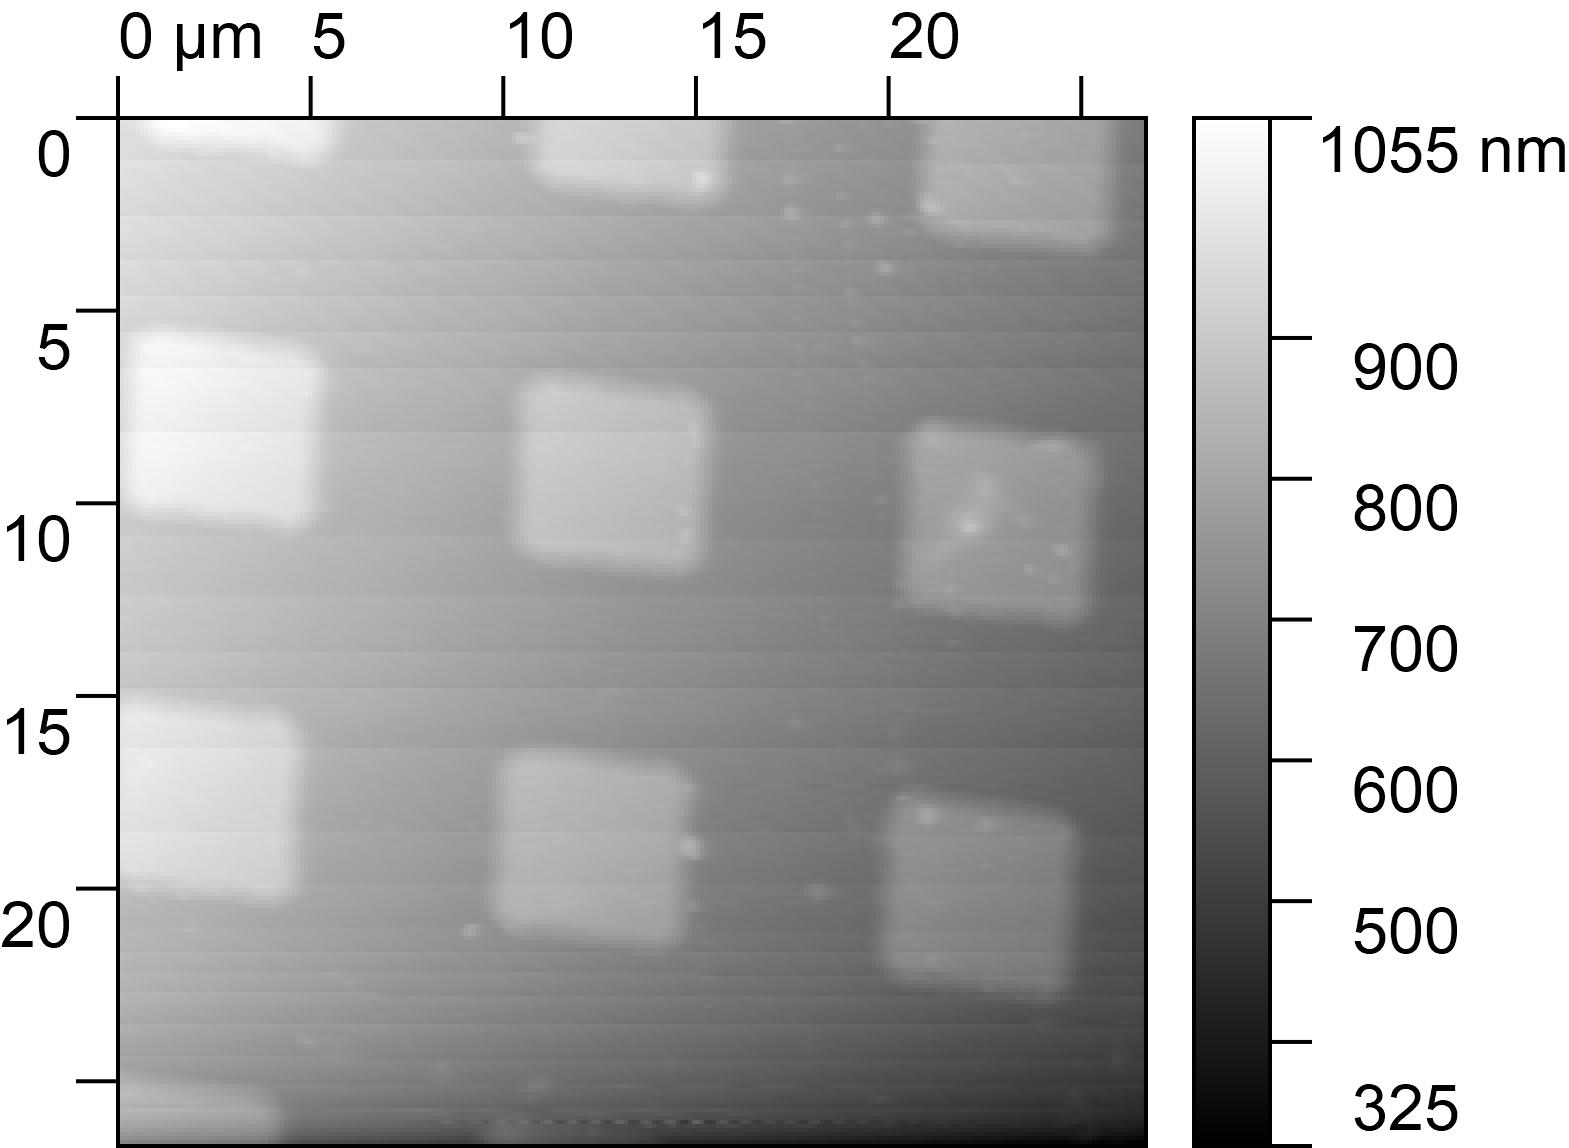
\includegraphics[width=.6\linewidth]{images/Kali/raw}
			\caption{Unbearbeitete Topografie der Kalibrierprobe.}
			\label{fig_kali_raw}
	\end{figure}

\subsubsection{Unsicherheiten}
	Folgende Unsicherheiten sind auf den Behältern der Cantilevers für die Federkonstante $c$ angegeben:
	\begin{description}
		\item[statischer Modus:] \SI{0.02}{N/m} - \SI{0.77}{N/m} % 0.395+-0.375
		\item[dynamischer Modus:] \SI{21}{N/m} - \SI{98}{N/m}
	\end{description}
	Alle weiteren Unsicherheiten bei der Kraft-Distanz-Spektroskopie werden als verschwinden gegenüber der Unsicherheit der Federkonstante angenommen.
\subsubsection{Kalibrierprobe}\label{sss_kali}
Die Skalierungsfaktoren der Achsen, wurden so gewählt, dass die Messung der Kalibrierprobe den Angaben bezüglich der Größe der Kalibrierquader aus \cite{Anleitung} entspricht.
Dies führt zu einem Faktor von $2/3$, mit dem in allen Raumrichtungen multipliziert wurde.
\begin{figure}[H]
			\subcaptionbox{Draufsicht \label{fig_kali_top}}{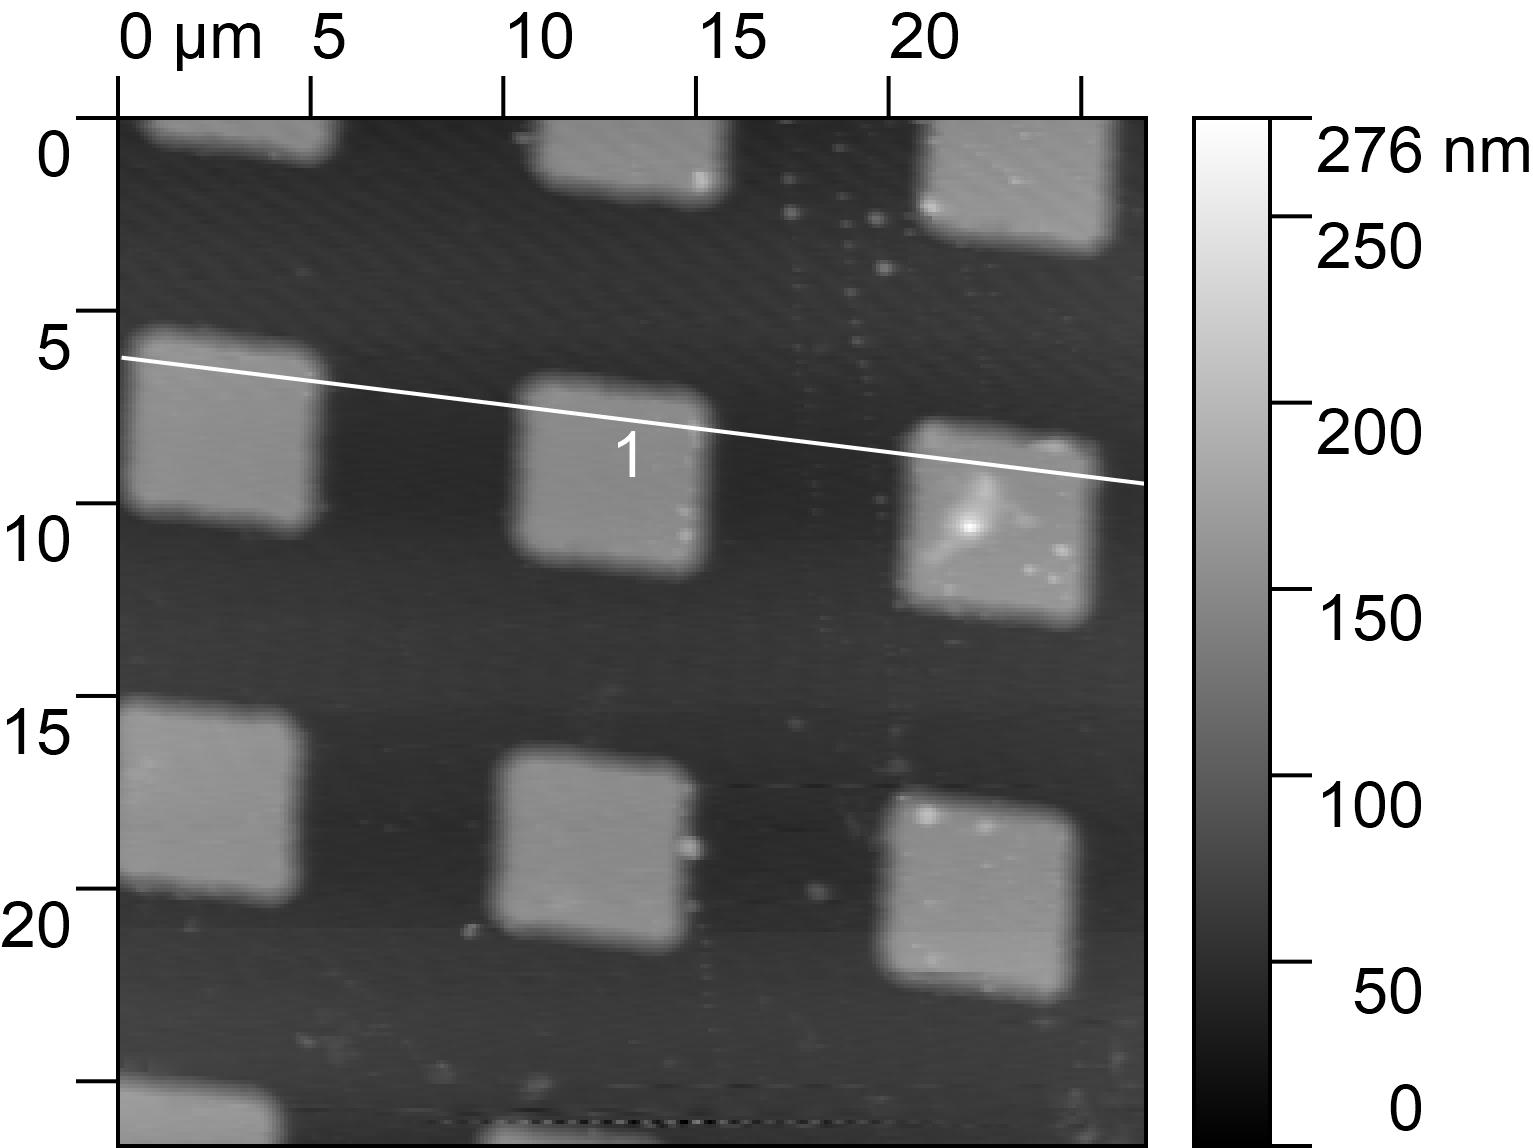
\includegraphics[width=.49\linewidth]{images/Kali/Top}}
			\subcaptionbox{3D-Sicht \label{fig_kali_3d}}{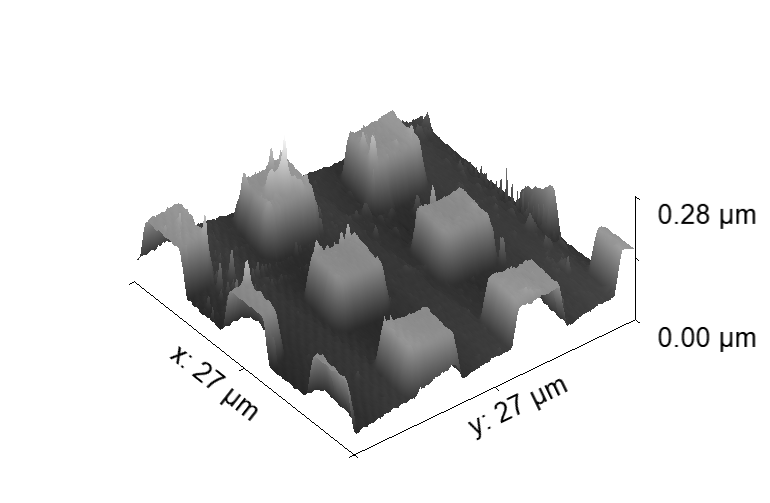
\includegraphics[width=.49\linewidth]{images/Kali/3D_fix}}
			\subcaptionbox{Profil entlang der Geraden 1 in \cref{fig_kali_top}.
			 \label{fig_kali_profil}}{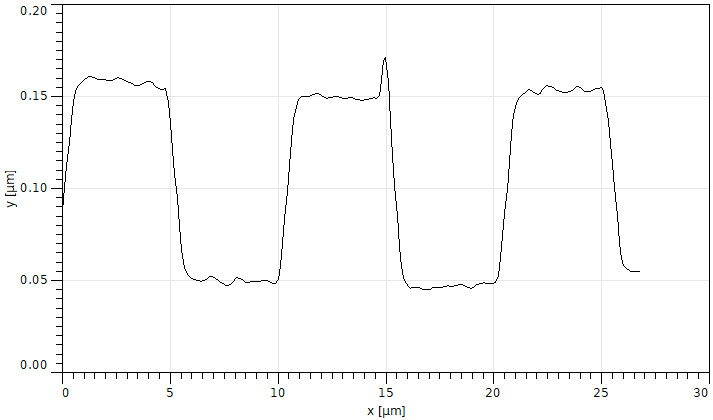
\includegraphics[width=.7\linewidth]{images/Kali/Profil}}
			\caption{Kalibrierprobe.}
\end{figure}
	% snap-offs 26.287, 28, 25.557, 35.1, 29.6 => 28.9
	Die Adhäsionskraft, welche an einem Punkt auf den Cantilever wirkt, während dieser sich von dem Material wegbewegt, lässt sich direkt aus dem Snap-off-Abstand $s$ und der Federkonstante mit \cref{eq_adh} bestimmen.
	In \cref{fig_kali_expl} ist exemplarisch eine gemessen Kraft-Abstands-Kurve dargestellt.
	Der Snap-off ist deutlich bei einem Abstand von ca. \SI{150}{nm} im Verlauf der blauen Kurve erkenntlich.
		Es folgt $F_\text{adh}=\SI{11.4+-10.8}{nN}$, wobei über die fünf gemessenen Hysteresen (Anhang: \crefrange{fig_kali_ds1}{fig_kali_ds5}) gemittelt wird.

\begin{equation}
			\label{eq_adh}
			F_\text{adh} = s \cdot c
	\end{equation}
%TODO Verweise

\begin {figure}[H]
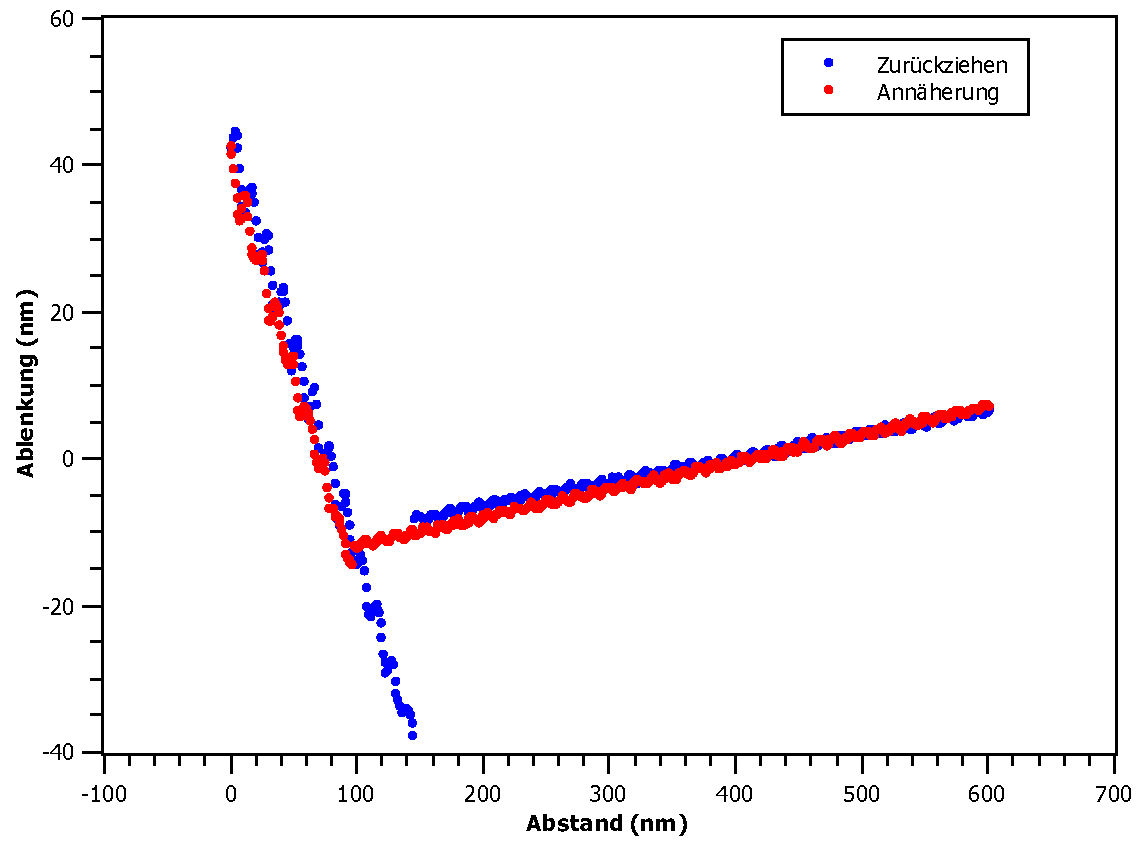
\includegraphics[width=.7\linewidth]{images/Kali/DS1}
\caption{Kraft-Abstands-Kurve der Kalibrierprobe auf einem der Quader.}
\label{fig_kali_expl}
\end{figure}

\subsubsection{Datenträgerproben}
%TODO Probe 3 (BR) war schwer Pits zu finden.
In \crefrange{fig_dvd}{fig_br} sind die gemessenen Topografien in Draufsicht und dreidimensionaler Sicht abgebildet.
Außerdem ist jeweils das Profil einer Geraden in der nicht vergrößerten Darstellung abgebildet.
Einzig bei Probe 3 war es notwendig mehrfach nach Spuren und Pits zu suchen.
Des Weiteren ist in der vergrößerten Topografie der dritten Probe kein Pit identifizierbar. %TODO Verweis?
Hier wurde möglicherweise auf einer Verunreinigung gemessen. %ja des ist diskus, aber da wär das so random und alleine

Analog zu \cref{sss_kali} lassen sich aus den Kraft-Abstands-Spektroskopie-Kurven (\cref{fig_dvd_ds}, \cref{fig_cd_ds} und \cref{fig_br_ds}) die Adhäsionskräfte der Datenträger bestimmen.
	Die resultierenden Adhäsionskräfte sind in \cref{tb_adh} aufgeführt.

\begin{table}[H]
		\centering
		\begin{tabular}{ c | c | c | c }
			 & Probe 1 & Probe 2 & Probe 3\\ \hline
			$F_\text{adh}$ & \SI{17.6+-16.7}{nN} & \SI{20.0+-19.0}{nN} &\SI{14.0+-13.3}{nN} \\
		\end{tabular}
		\caption{Adhäsionskräfte, die auf die Spitze des Cantilevers wirken, bei Kraft-Abstands-Spektroskopie.}
		\label{tb_adh}
\end{table}

	Die Spurbreite $b_\text{Spur}$ des jeweiligen Datenträgers ergibt sich gemittelt aus den in \cref{fig_dvd_profil}, \cref{fig_cd_profil} bzw. \cref{fig_br_profil} gemessenen Abständen mehrer Spuren.
	Der Abstand wird trivialerweise durch die Anzahl der Spuren dividiert.
	Es folgen die Spurbreiten in \cref{tb_spur}.
	Analog lassen sich Pit-Länge $l_\text{Pit}$ , Pit-Breite $b_\text{Pit}$ und Pit-Tiefe $t_\text{Pit}$ bestimmen.
	Diese sind ebenfalls in \cref{tb_spur} aufgeführt.

\begin{table}[H]
		\centering
		\begin{tabular}{ c | c | c | c }
			 & Probe 1 & Probe 2 & Probe 3\\ \hline
			$b_\text{Spur}$ & \SI{690}{nm} & \SI{1510}{nm} &\SI{330}{nm} \\
			$l_\text{Pit}$ & \SI{530}{nm} & \SI{873}{nm} &\SI{170}{nm} \\
			$b_\text{Pit}$ & \SI{390}{nm} & \SI{682}{nm} &\SI{321}{nm} \\
			$t_\text{Pit}$ & \SI{63}{nm} & \SI{48}{nm} &\SI{41}{nm} \\
		\end{tabular}
		\caption{Spurbreite $b_\text{Spur}$, Pit-Länge $l_\text{Pit}$, Pit-Breite $b_\text{Pit}$, Pit-Tiefe $t_\text{Pit}$ der jeweiligen Datenträger 1-3.
		Die Unsicherheiten werden jeweils mit \SI{5}{\%} abgeschätzt.
		Da nicht ausgeschlossen werden kann dass ein Großteil dieses Fehlers systematisch ist, wird für die Mittelwerte kein veringerter Fehler angenommen.}
		\label{tb_spur}
	\end{table}

	% 1) DVD
	% 2) CD
	% 3) BR

	%TODO die 3Seiten Graphik fliegen hier noch bisschen wasted rum
\begin{figure}[H]
			\subcaptionbox{Draufsicht \label{fig_dvd_top}}{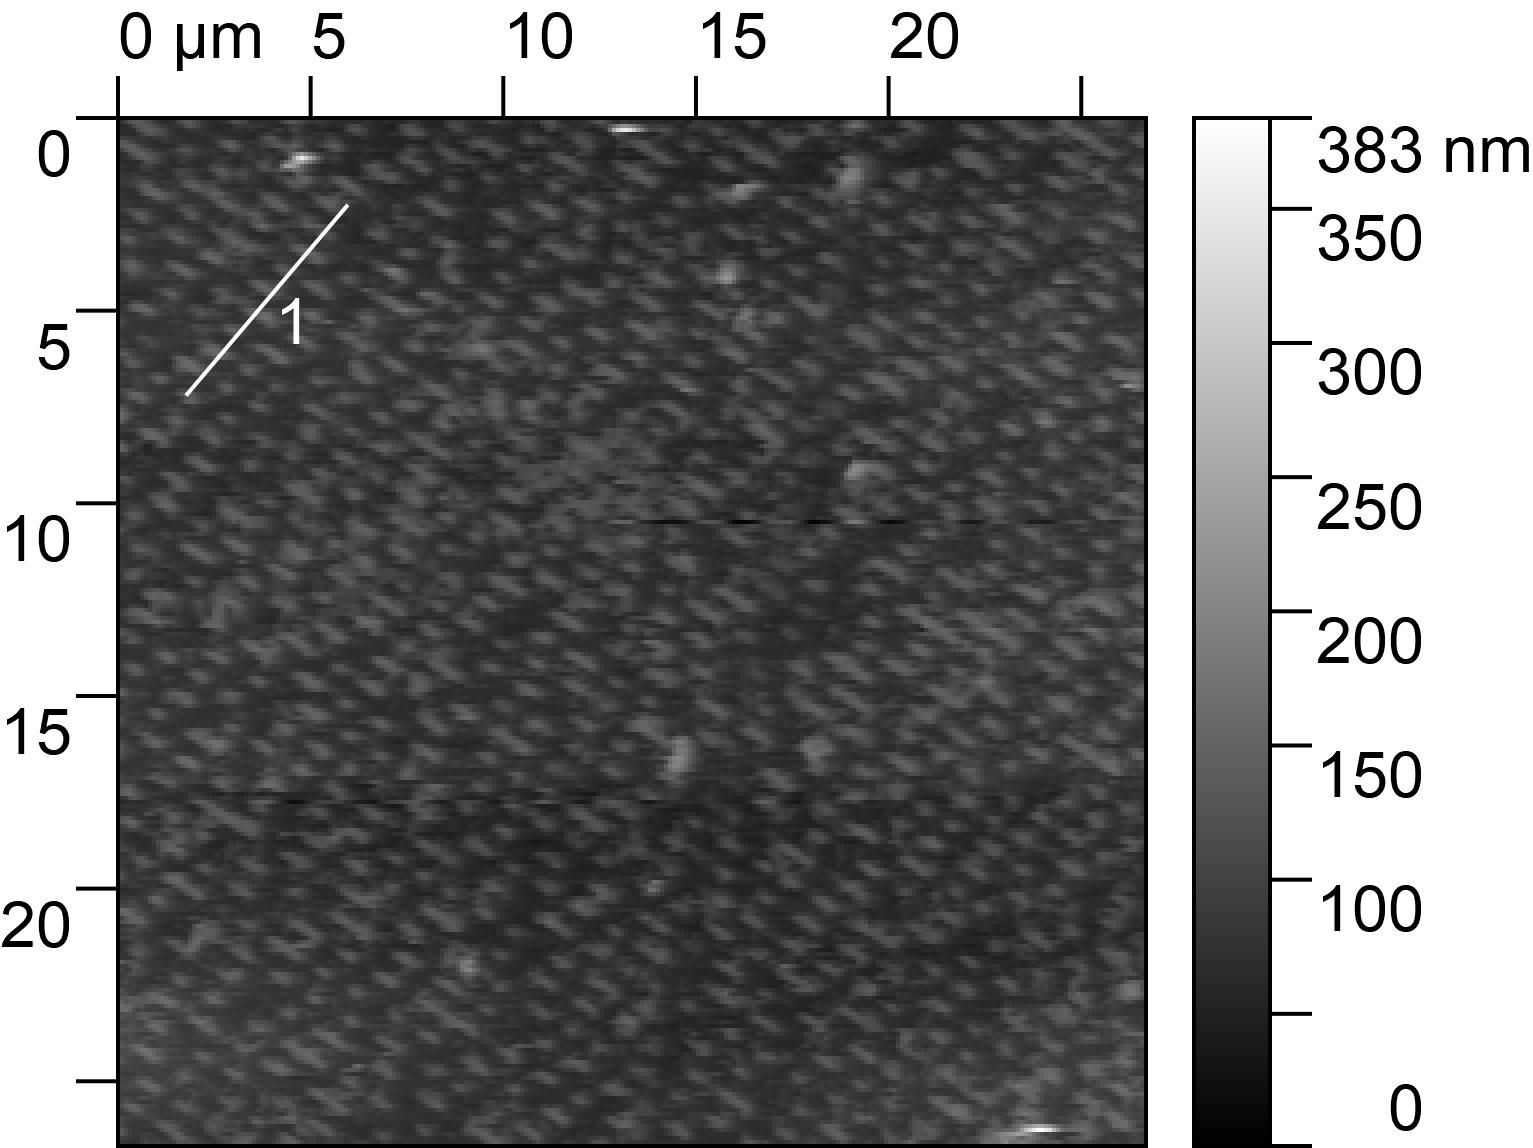
\includegraphics[width=.49\linewidth]{images/DVD/Top}}
			\subcaptionbox{3D-Sicht \label{fig_dvd_3d}}{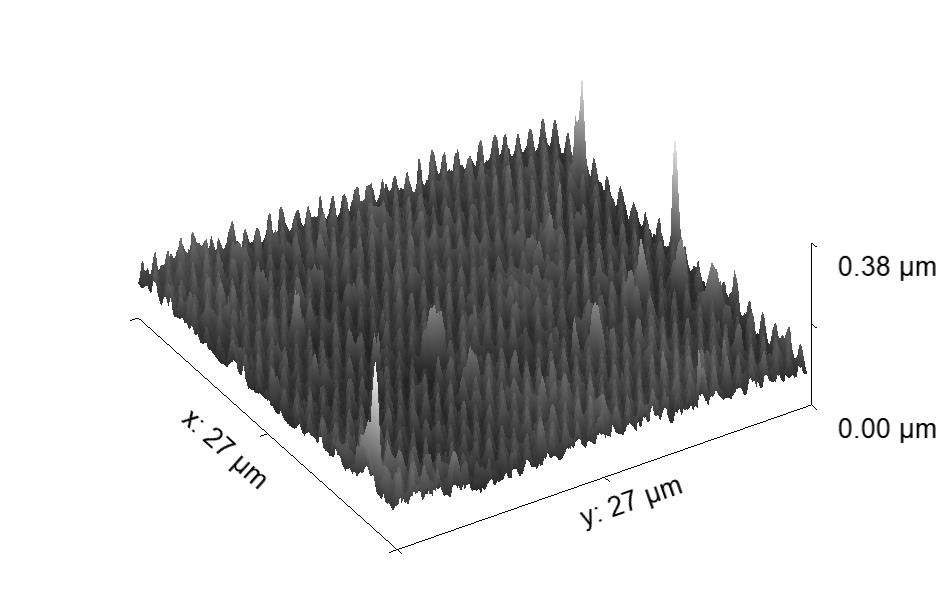
\includegraphics[width=.49\linewidth]{images/DVD/3D_fix}}
			\subcaptionbox{Vergrößerte Draufsicht \label{fig_dvd_top_zoom}}{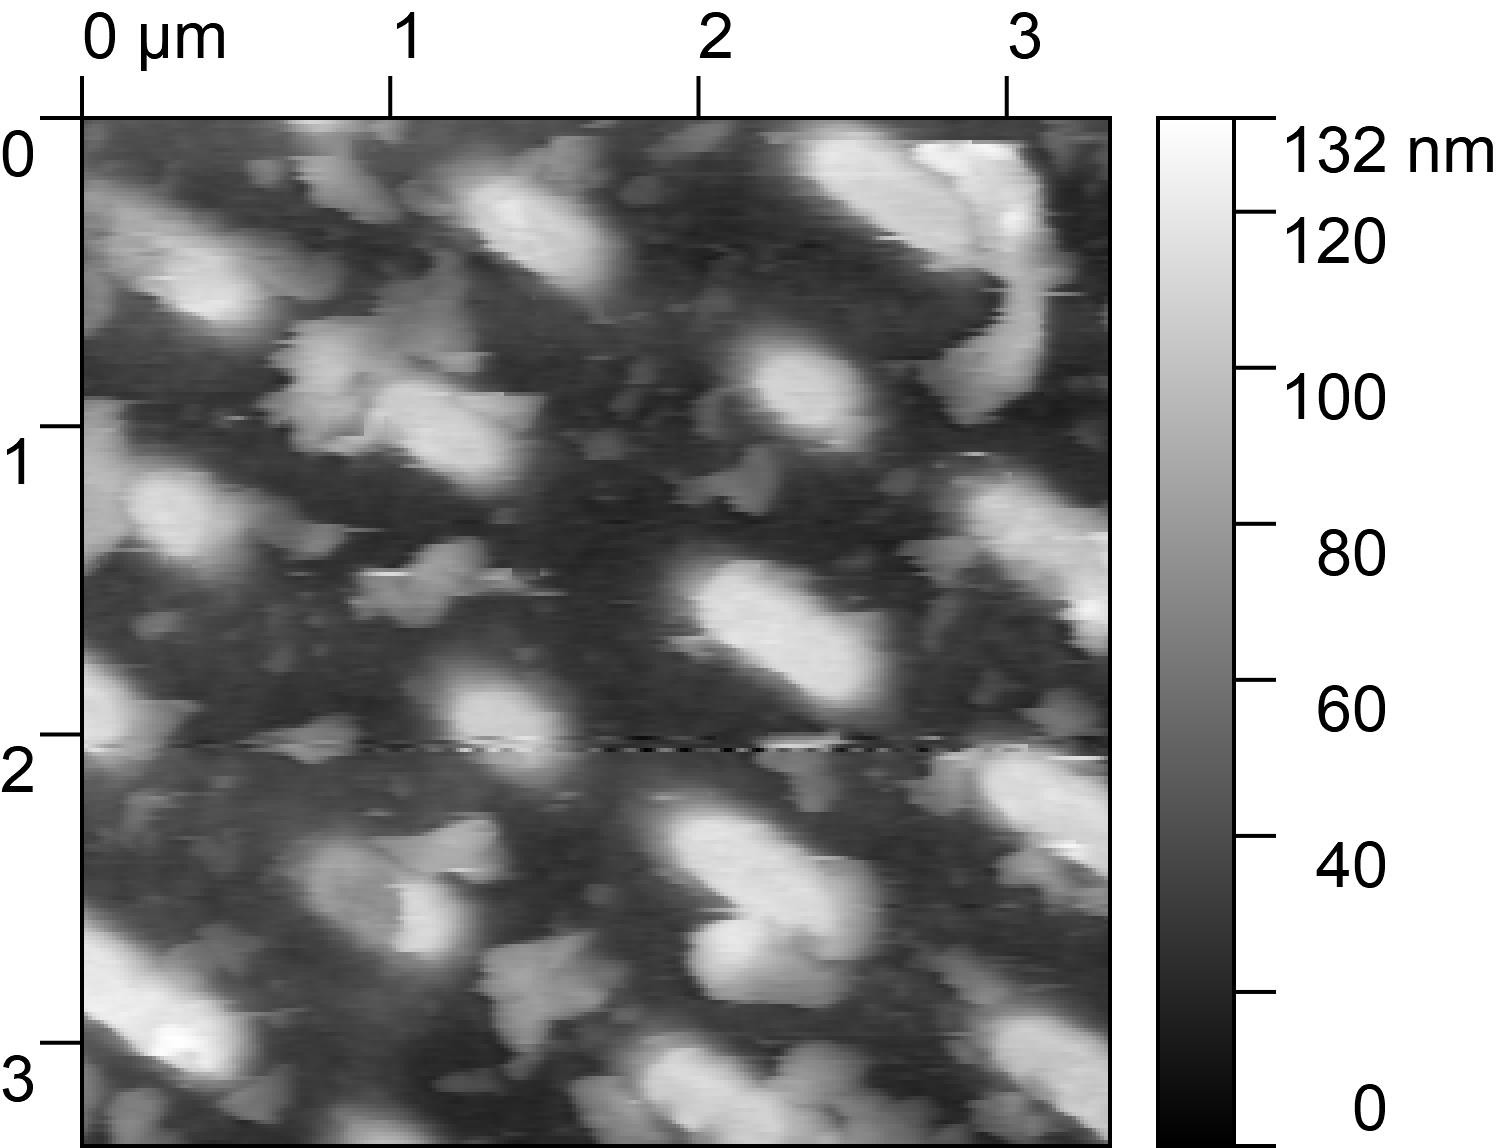
\includegraphics[width=.49\linewidth]{images/DVD/Top_zoom}}
			\subcaptionbox{Vergrößerte 3D-Sicht \label{fig_dvd_3d_zoom}}{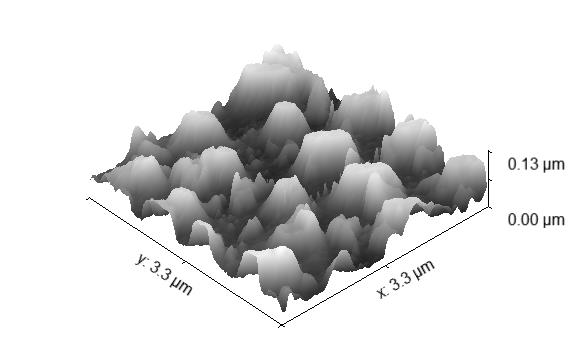
\includegraphics[width=.49\linewidth]{images/DVD/3D_zoom}}
			\subcaptionbox{Profil entlang der Geraden 1 in \cref{fig_dvd_top}.
			  Der gemessene Abstand zwischen den zwei Senkrechten beträgt \SI{5.48}{\mu m}.
			 \label{fig_dvd_profil}}{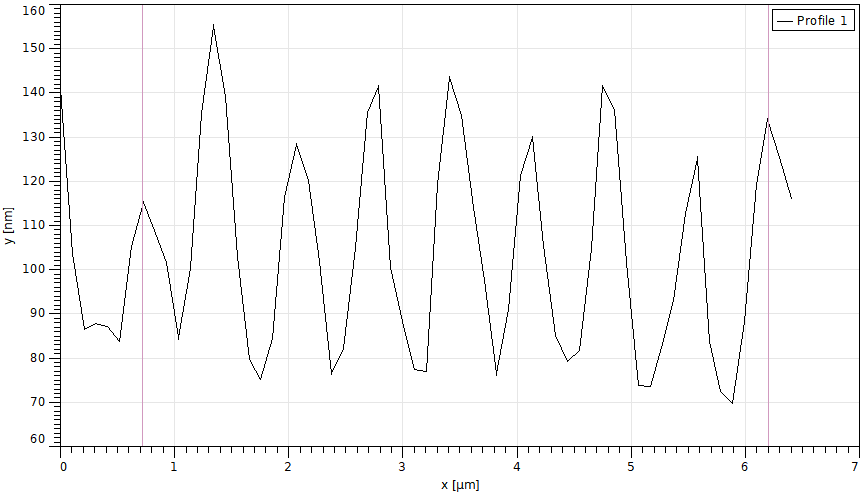
\includegraphics[width=.9\linewidth]{images/DVD/Profil}}
			\caption{Probe 1.}
			\label{fig_dvd}
\end{figure}


\begin{figure}[H]
			\subcaptionbox{Draufsicht \label{fig_cd_top}}{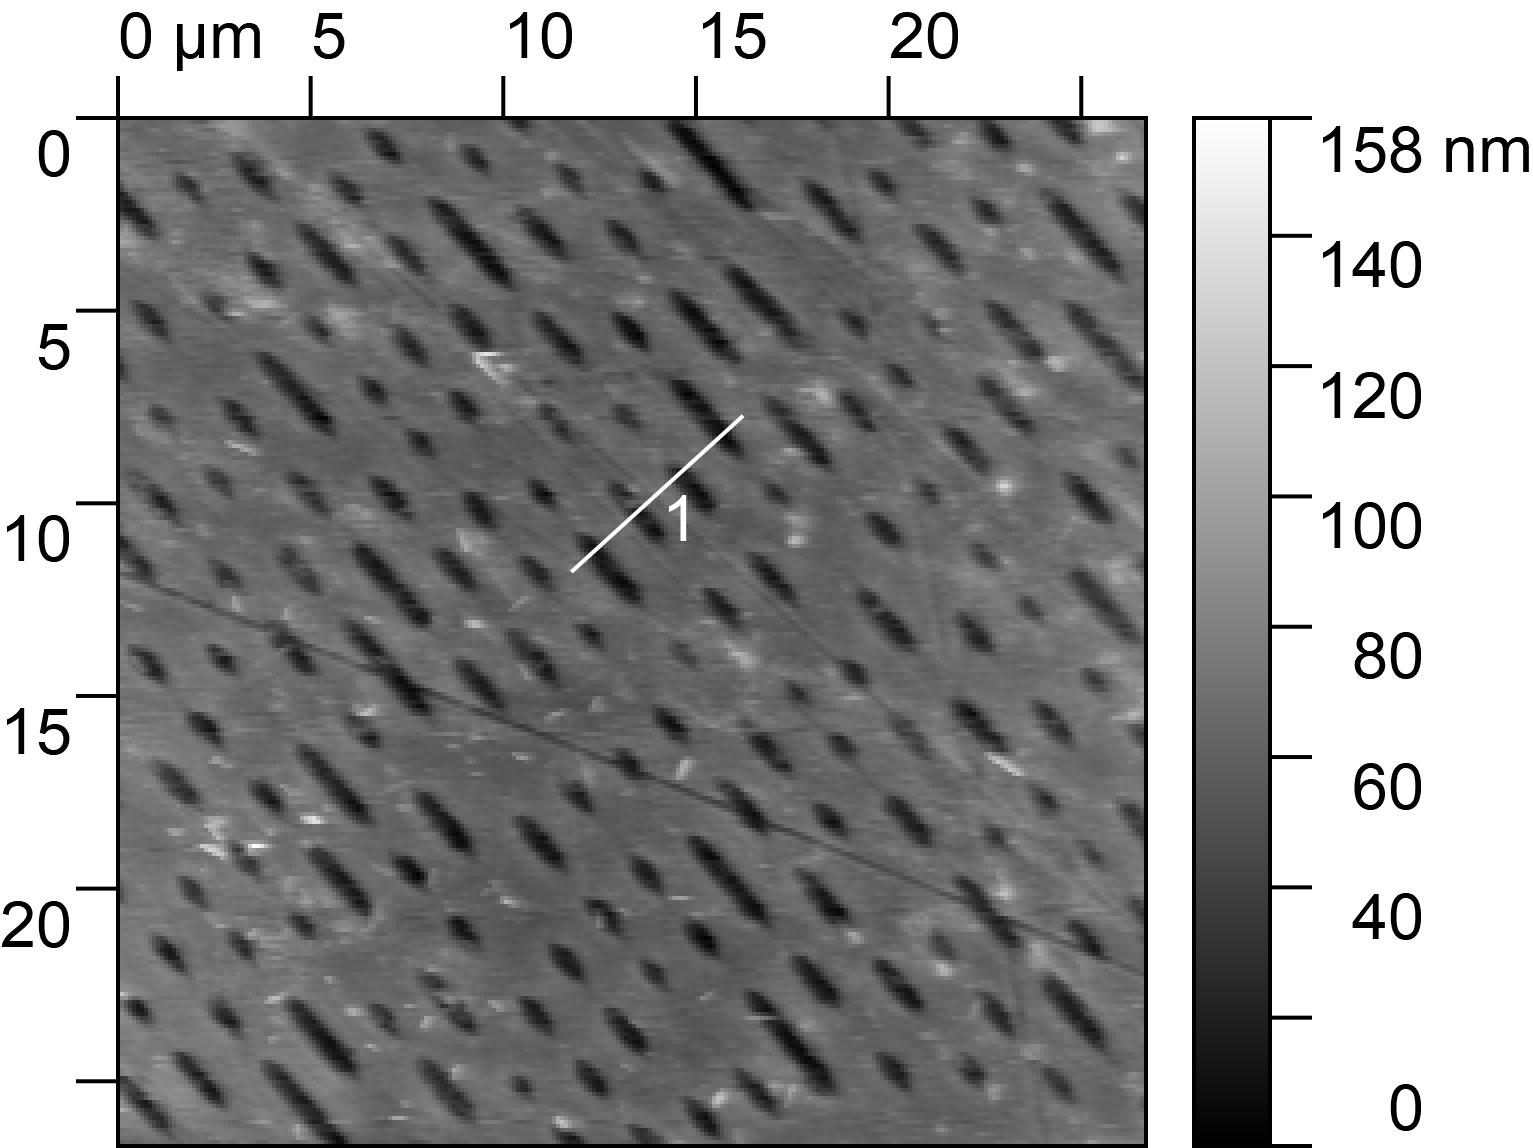
\includegraphics[width=.49\linewidth]{images/CD/Top}}
			\subcaptionbox{3D-Sicht \label{fig_cd_3d}}{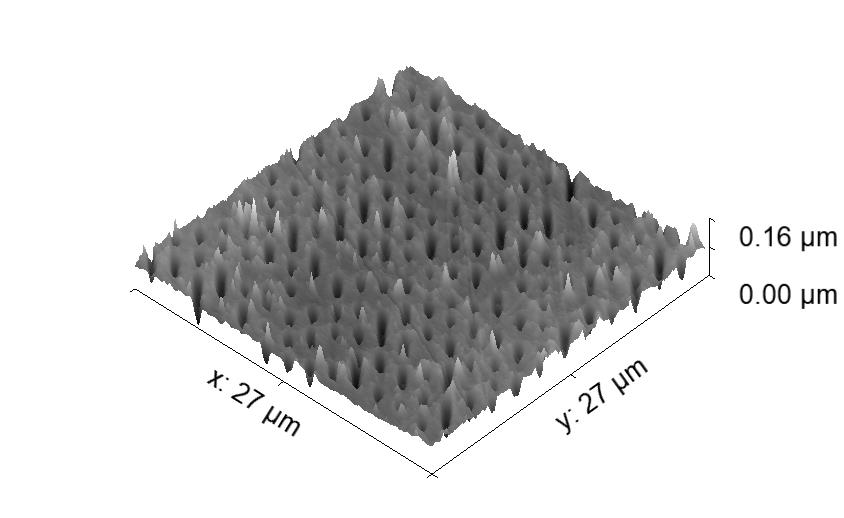
\includegraphics[width=.49\linewidth]{images/CD/3D_fix}}
			\subcaptionbox{Vergrößerte Draufsicht \label{fig_cd_top_zoom}}{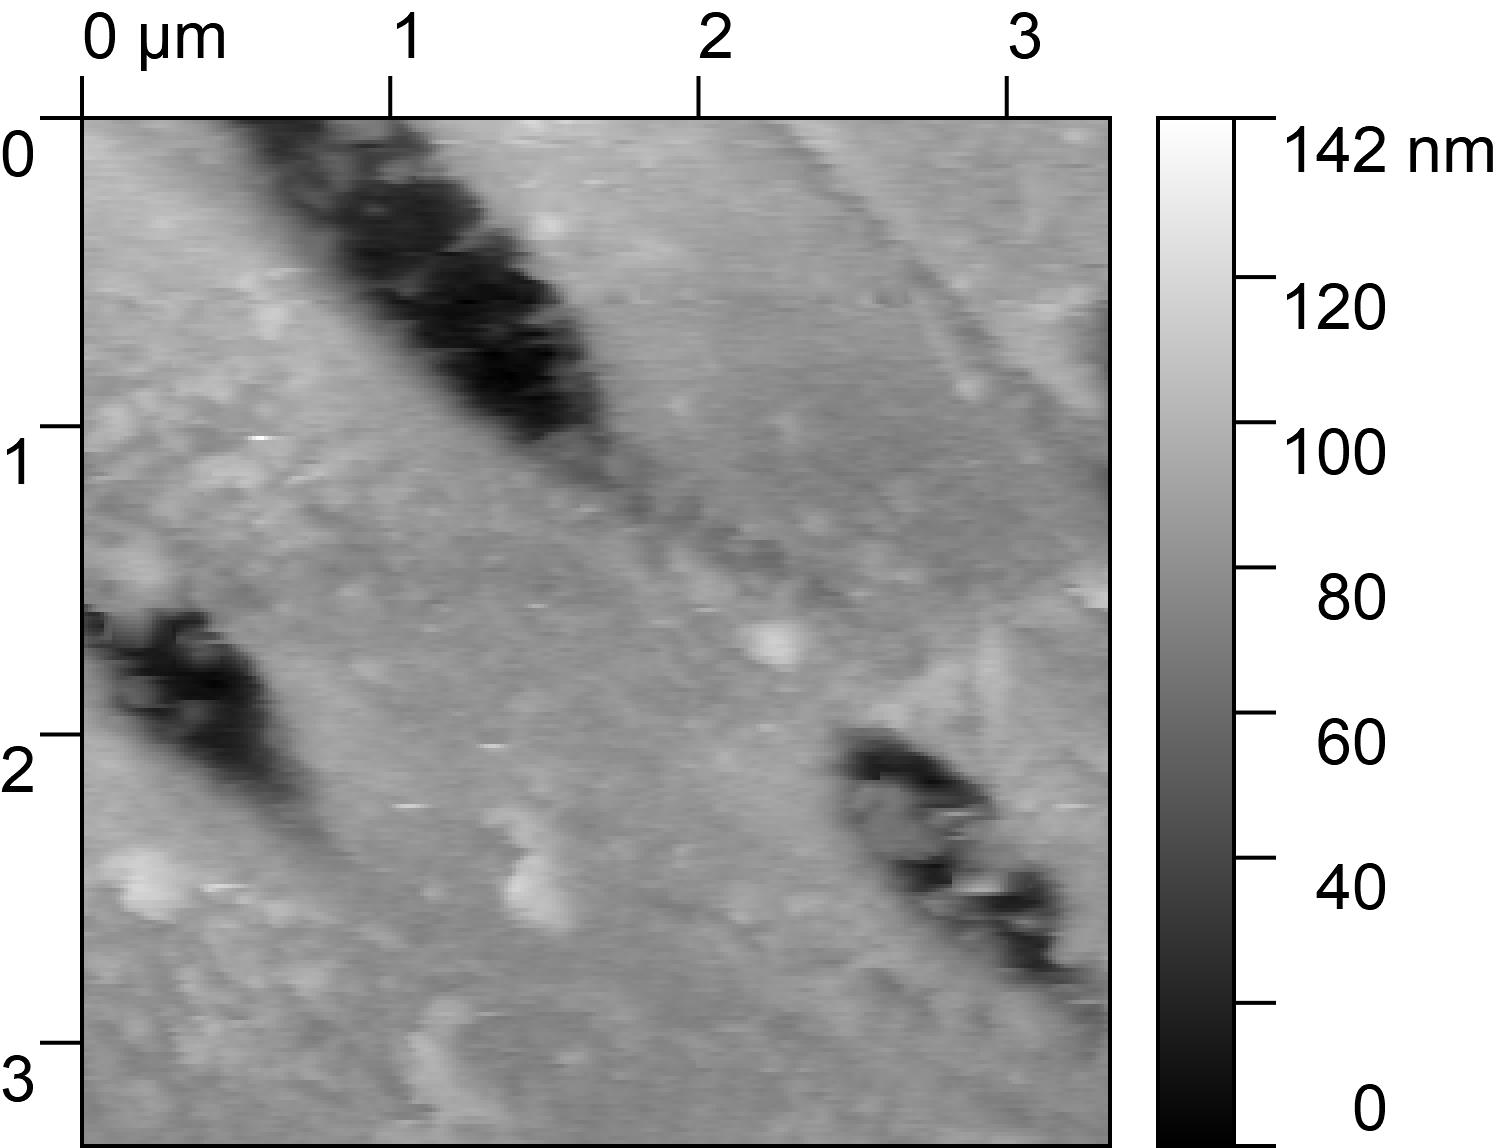
\includegraphics[width=.49\linewidth]{images/CD/Top_zoom}}
			\subcaptionbox{Vergrößerte 3D-Sicht \label{fig_cd_3d_zoom}}{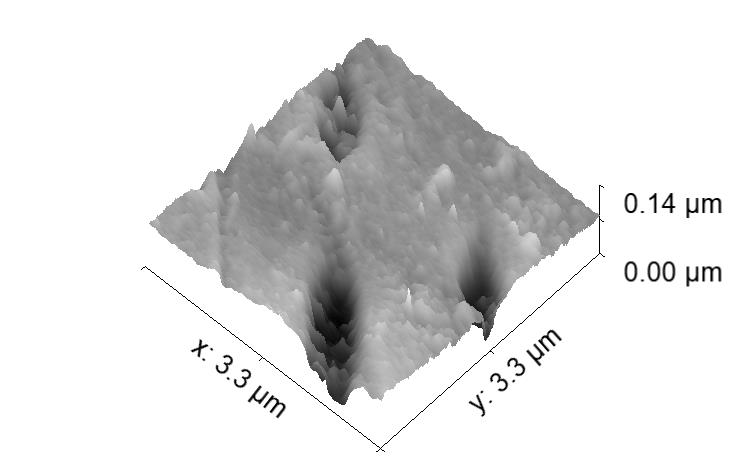
\includegraphics[width=.49\linewidth]{images/CD/3D_zoom_fix}}
			\subcaptionbox{Profil entlang der Geraden 1 in \cref{fig_cd_top}. Der gemessene Abstand zwischen den zwei Senkrechten beträgt \SI{4.535}{\mu m}. % Die Tiefe des Minimums bei $x\approx\SI{5.3}{\mu m}$ beträgt \SI{58.5}{nm}.
			 \label{fig_cd_profil}}{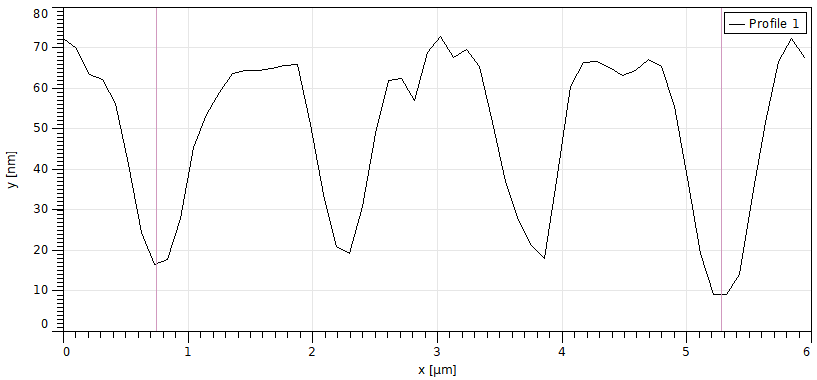
\includegraphics[width=.95\linewidth]{images/CD/Profil}}
			\caption{Probe 2.}
			\label{fig_cd}
\end{figure}

\begin{figure}[H] %Hier finde ich die Vergrößerte Sicht sehr merkwürdig (und eigentlich auch die nicht-vergrößerte)
			\subcaptionbox{Draufsicht \label{fig_br_top}}{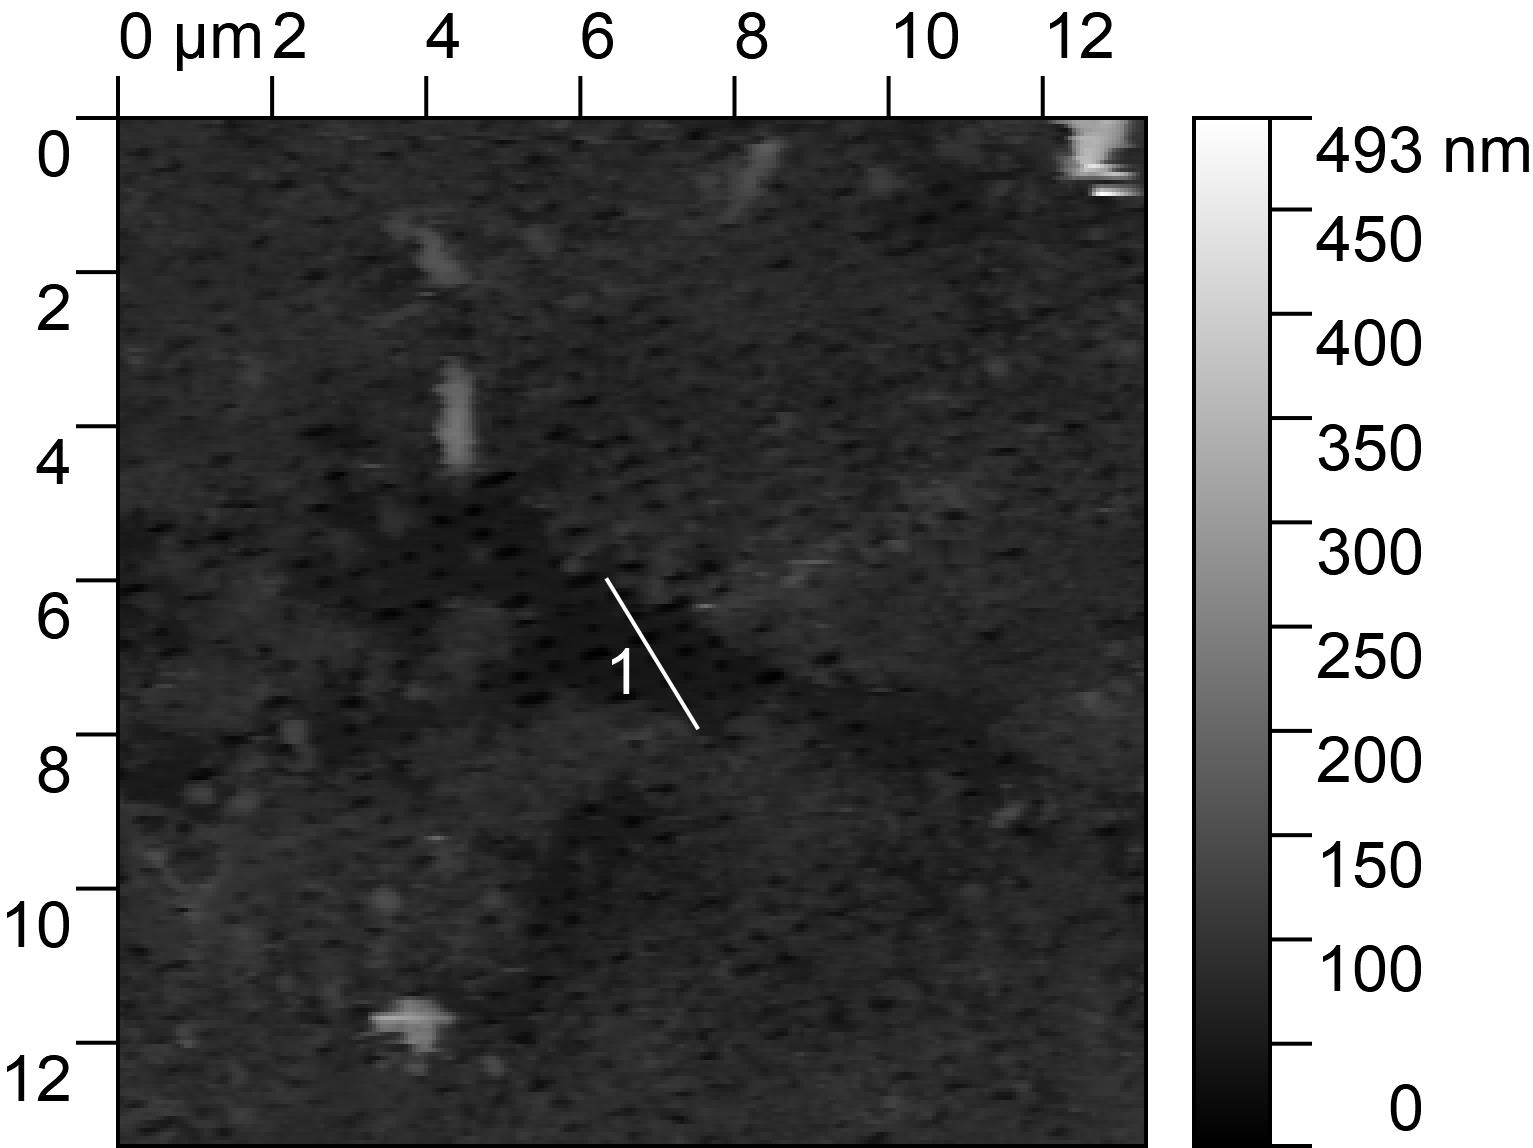
\includegraphics[width=.49\linewidth]{images/BR/Top}}
			\subcaptionbox{3D-Sicht \label{fig_br_3d}}{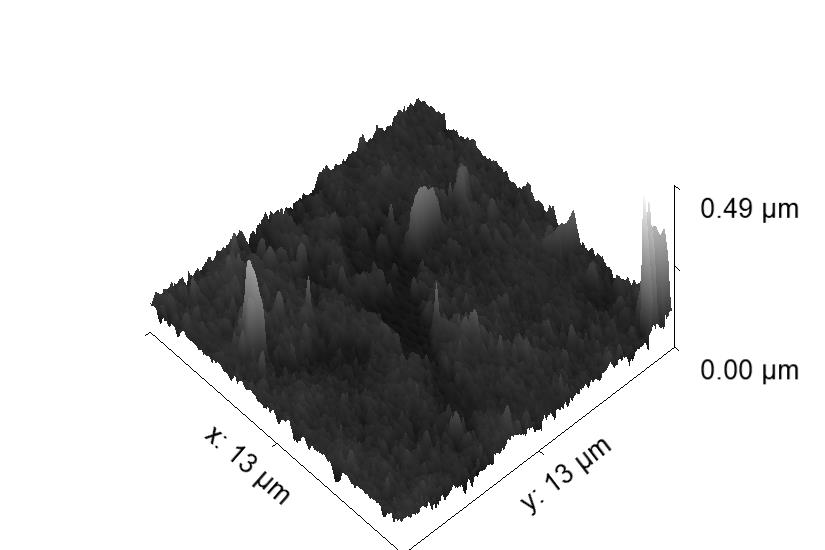
\includegraphics[width=.49\linewidth]{images/BR/3D_fix}}
			\subcaptionbox{Vergrößerte Draufsicht \label{fig_br_top_zoom}}{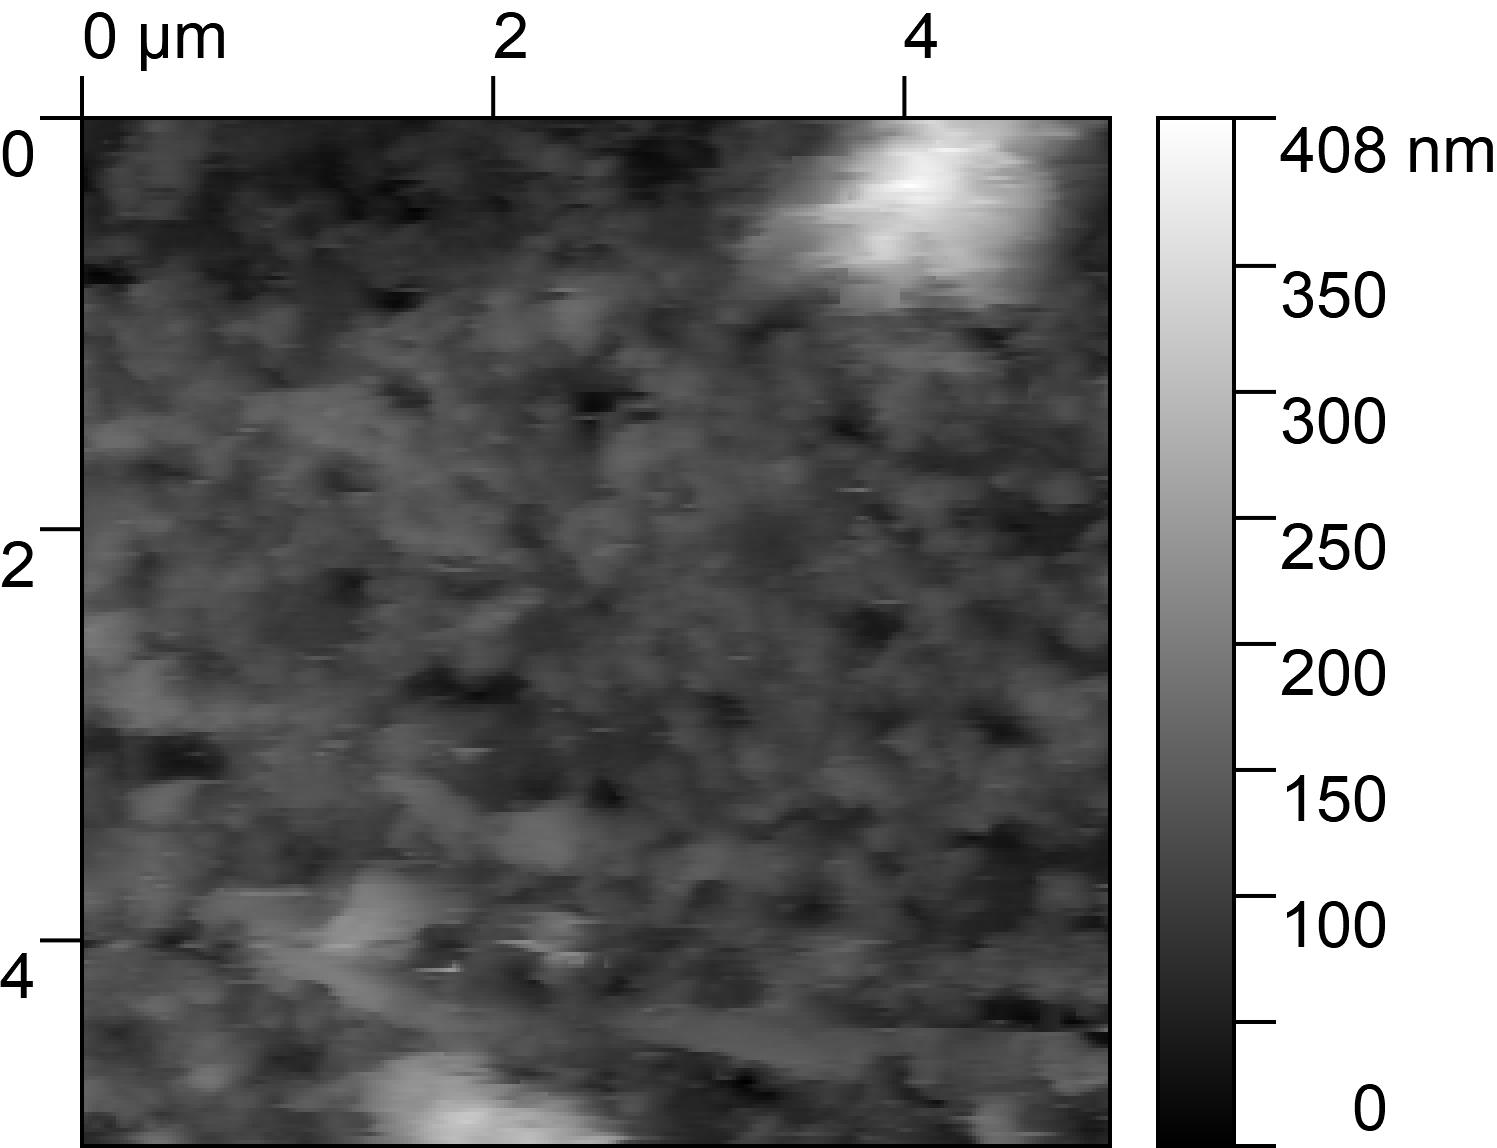
\includegraphics[width=.49\linewidth]{images/BR/Top_zoom}}
			\subcaptionbox{Vergrößerte 3D-Sicht \label{fig_br_3d_zoom}}{\includegraphics[width=.49\linewidth]{images/BR/3D_zoom_fix}}
			\subcaptionbox{Profil entlang der Geraden 1 in \cref{fig_br_top}.
			Der gemessene Abstand zwischen den zwei Senkrechten beträgt \SI{1.64}{\mu m}.
				%Die Tiefe des Minimums bei $x\approx\SI{1}{\mu m}$ beträgt \SI{39.3}{nm}.
			\label{fig_br_profil}}{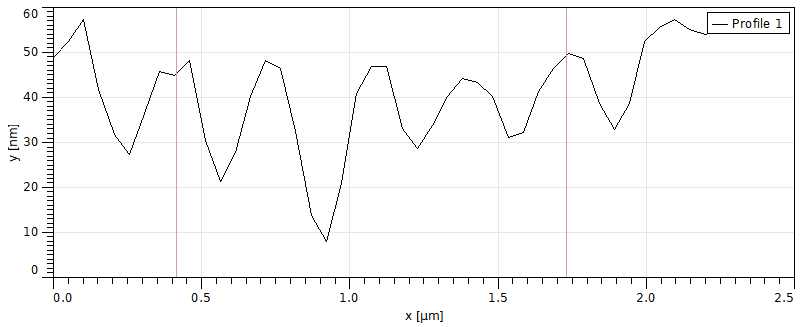
\includegraphics[width=.99\linewidth]{images/BR/Profil}}
			\caption{Probe 3.}
			\label{fig_br}
\end{figure}

\subsubsection{TGT1-Probe}

Im dynamischen Modus ist in der Topografie zunächst kein periodisches Spitzenmuster erkennbar.
Erst nach Optimierung der Parameter für den PID-Regler lassen sich Strukturen erkennen (\cref{fig_tgt}).

\begin{figure}[H]
			\subcaptionbox{Draufsicht
			 \label{fig_tgt_top}}{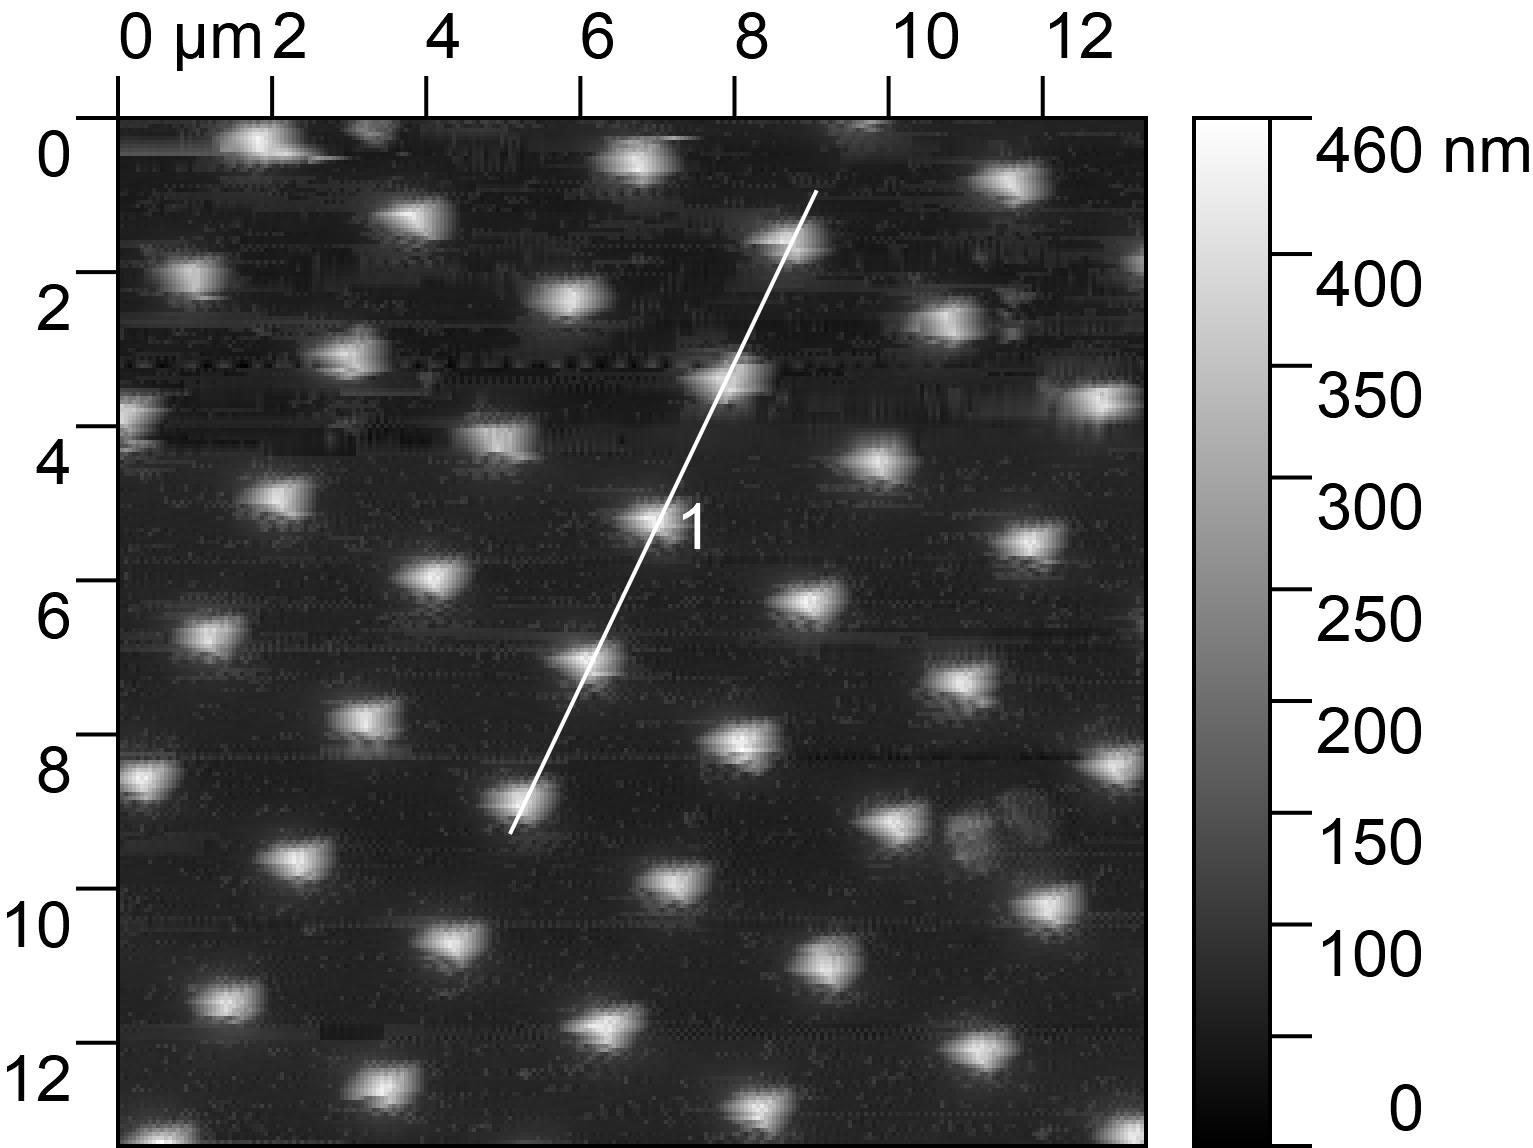
\includegraphics[width=.49\linewidth]{images/TGT/Top}}
			\subcaptionbox{3D-Sicht
			\label{fig_tgt_3d}}{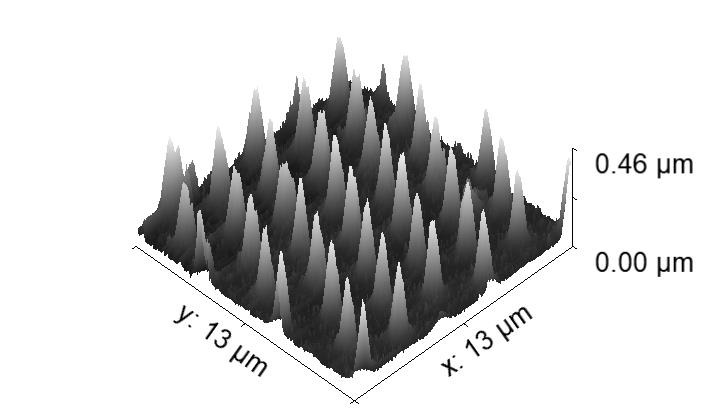
\includegraphics[width=.49\linewidth]{images/TGT/3D_fix}}
			\subcaptionbox{Profil entlang der Geraden 1 in \cref{fig_tgt_top}.
			\label{fig_tgt_profil}}{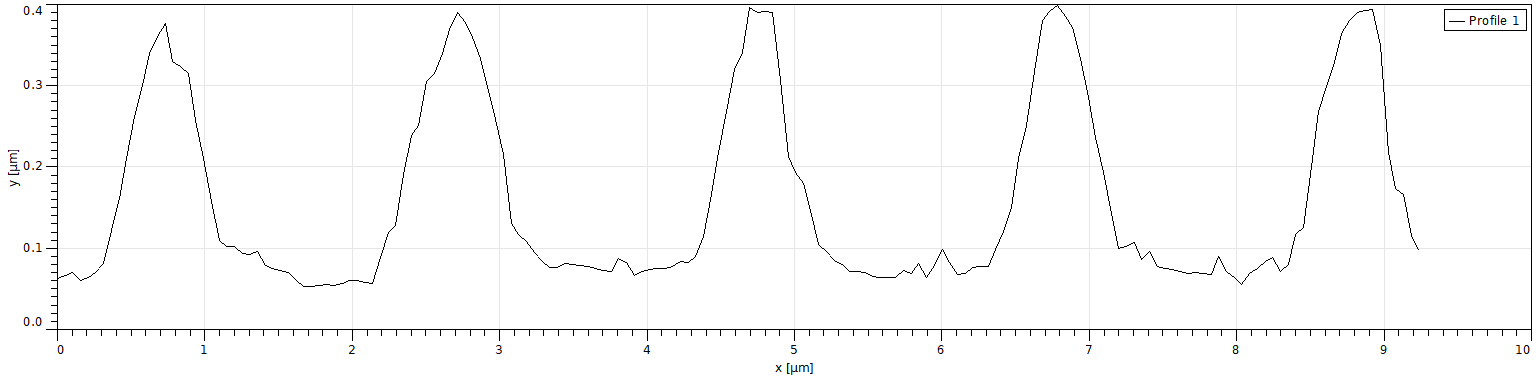
\includegraphics[width=.99\linewidth]{images/TGT/Profil}}
			\caption{TGT1 Probe.}
			\label{fig_tgt}
\end{figure}

Aus dem Profil einer gemessenen Spitze in \cref{fig_tgt_profil_zoom} lässt sich mittels einer Anpassung an einen Kreis der Radius der Spitze des Cantilevers bestimmen.
Es ergibt sich ein Radius $r=\SI{1.204 +-0.016}{\mu m}$.

\begin{figure}[H]
			\subcaptionbox{Draufsicht
			 \label{fig_tgt_top_zoom}}{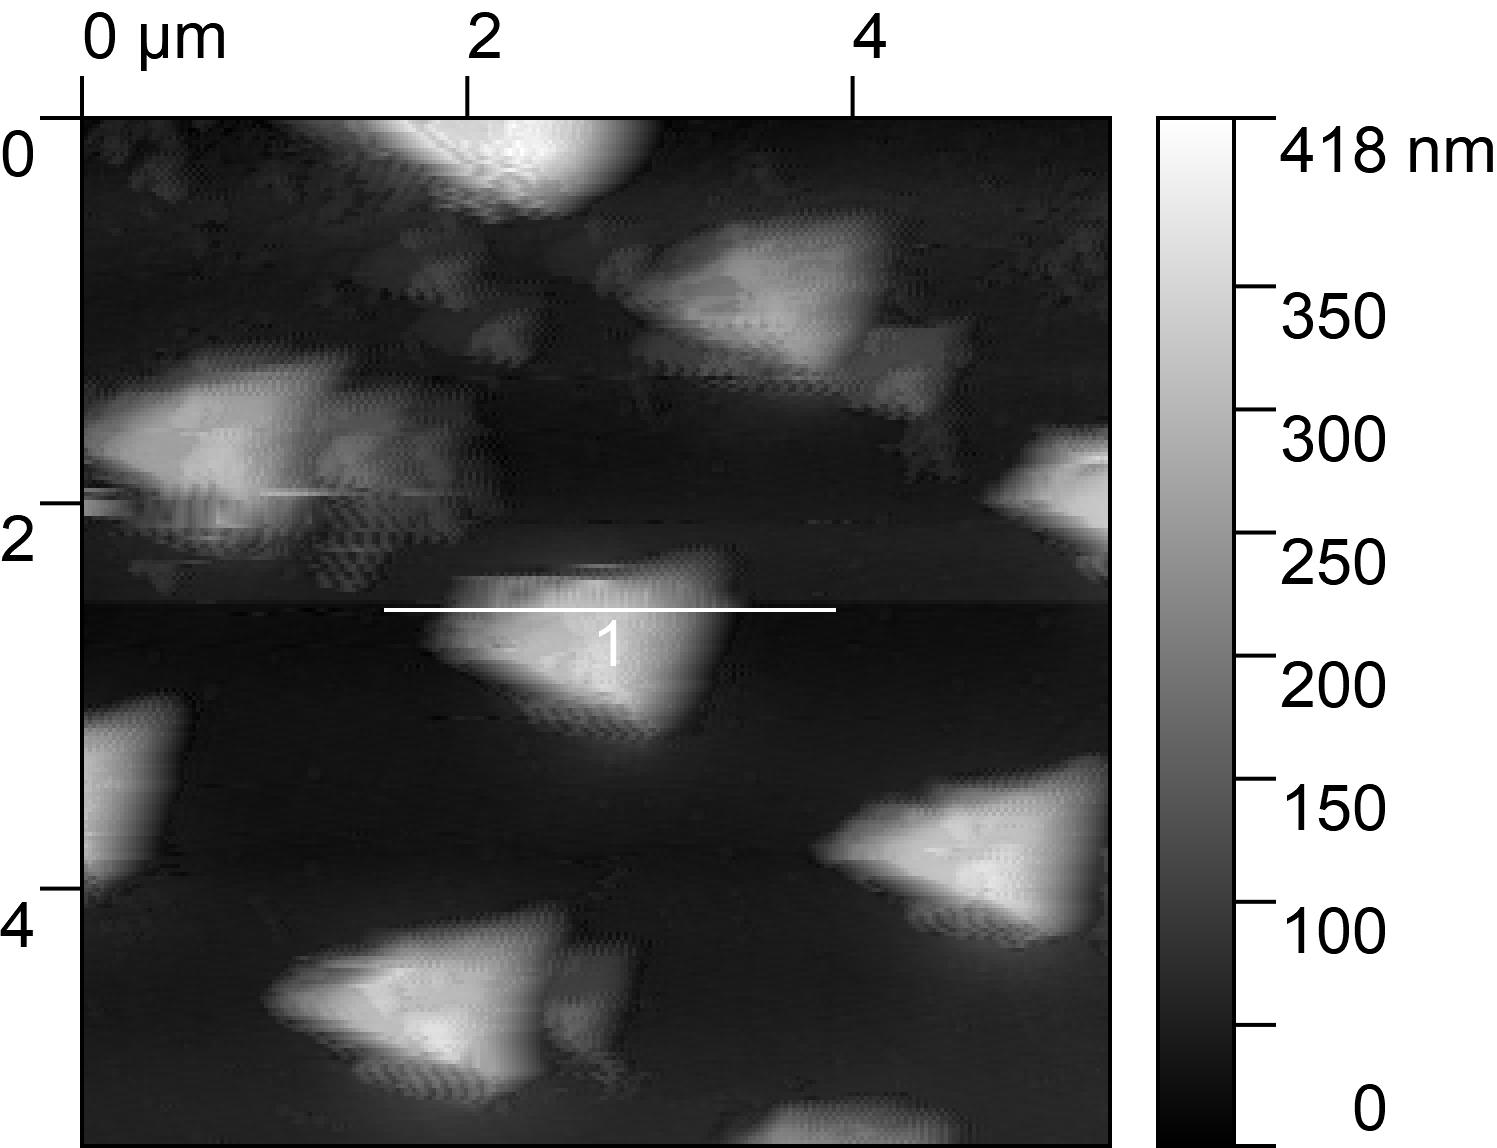
\includegraphics[width=.49\linewidth]{images/TGT/Top_zoom}}
			\subcaptionbox{3D-Sicht
			\label{fig_tgt_3d_zoom}}{\includegraphics[width=.49\linewidth]{images/TGT/3D_zoom_fix}}
			\subcaptionbox{Profil entlang der Geraden 1 in \cref{fig_tgt_top_zoom}.
			Die rote Funktion ist ein Kreis mit dem Radius $r= \SI{1.204 +-0.016}{\mu m}$.
			\label{fig_tgt_profil_zoom}}{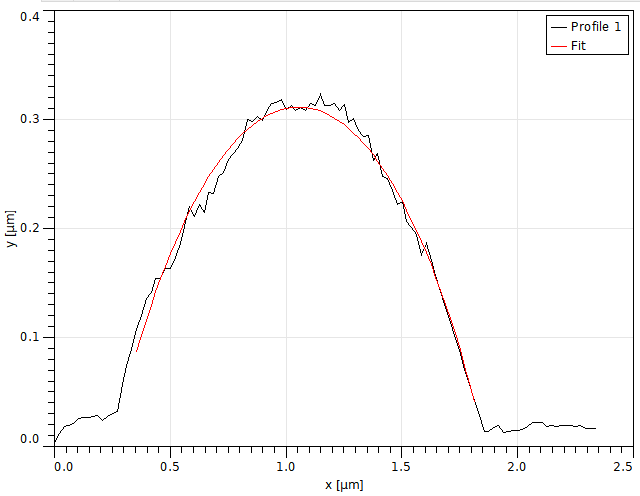
\includegraphics[width=.6\linewidth]{images/TGT/Profil_zoom}}
			\caption{TGT1 Probe.}
			\label{fig_tgt_zoom}
\end{figure}

		\subsection{Diskussion}
	%TODO Dreieck form von TGT1 disksus?
	\subsubsection{Zuordnung der Datenträger}
	\begin{table}[H]
		\centering
		\begin{tabular}{ c | c | c | c}
			&CD \cite{CD}&DVD \cite{DVD}&Blu-ray \cite{blu}\\ \hline
			Literaturwerte & \SI{1600}{\nano \meter} & \SI{740}{\nano \meter}& \SI{320}{\nano \meter}\\
			Probennummer & 2 & 1 & 3\\
			Messwert & \SI{1510+-75,5}{\nano \meter} & \SI{690 +-34,5}{\nano \meter} & \SI{330 +- 16,5}{\nano \meter}\\
		\end{tabular}
		\caption{Spurabstände von CD, DVD, und Blu-ray Disc gemäß Literaturwerten und zugeordneten Proben.}
		\label{tb_lit_Spurabstände}
	\end{table}
	In \cref{tb_lit_Spurabstände} wurden die Proben anhand von Literaturwerten den verschiedenen optischen Speichermedien zugeordnet.
	Dies gelingt für die Blu-ray Disc innerhalb der Unsicherheit und für CD und DVD innerhalb der doppelten Unsicherheit.
	Die Abweichungen können unter anderem dadurch zustande kommen, dass nicht sichergestellt werden kann, ob die Gerade, über die das Profil gebildet wurde, exakt senkrecht zur Spur liegt.
	Demnach lässt sich festhalten, dass die Raster-Kraft-Mikroskopie im Kontaktmodus für Strukturen in der Größenordnung von einigen hundert Nanometern ein geeignetes Verfahren ist.
	Da die z-Achse hier jedoch im Bereich von einigen zehn Nanometern liegt, lässt sich jedoch feststellen, dass das Verfahren auch noch kleinere Strukturen auflöst, allerdings kann hier aufgrund der Probentopografie nicht festgestellt werden, ob Strukturen dieser Größe auch in x- und y-Richtung aufgelöst werden können.
	Es ist außerdem festzustellen, dass die Probe, die aus der Beschichtung des Speichermediums bestand, die DVD ist, da dies die einzige ist, bei der die Pits als Berge auftreten (vgl. \cref{fig_dvd_3d_zoom}).

	\subsubsection{Spitzenradius}
	Die Bestimmung des Spitzenradius führte zu einem Wert von \SI{1,204 +- 0,016}{\micro \meter}.
	Dies steht im deutlichen Widerspruch zu den Angaben des Herstellers von \SI{7}{\nano \meter} aus dem Programm zur Bedienung des Mikroskops \enquote{Nanosurf Easyscan 2}.
	Diese Feststellung muss darauf zurückgeführt werden, dass entweder die Cantilever-Spitze oder die Probenspitzen einen deutlich größeren Radius haben, als der Hersteller angibt.
	Dies kann sowohl herstellungsbedingt sein als auch durch Beschädigung zustande gekommen sein.
	Außerdem fällt in \cref{fig_tgt_top_zoom} auf, dass die Spitzen eine dreieckige Form haben und in \cref{fig_tgt_3d_zoom} nicht sonderlich spitz zulaufen und gleichzeitig selten im Profil einen Halbkreis bilden.
	Es ist allerdings eine Regelmäßigkeit zu erkennen, woraus geschlossen werden kann, dass die Cantilever-Spitze entweder tatsächlich diese unregelmäßige Form hat, oder eine Verzerrung durch den PID-Regler stattfindet.
	\subsubsection{Adhäsion}

	\begin{table}[H]
		\centering
		\begin{tabular}{ c | c | c| c | c }
			 & Kalibrierprobe & CD & DVD & Blu-ray\\ \hline
			$F_\text{adh}$ & \SI{11.4+-10.8}{nN} & \SI{20,0+-19,0}{\nano \newton}& \SI{17,6 +- 16,7}{\nano \newton}& \SI{14,0+-13,3}{\nano \newton} \\
		\end{tabular}
		\caption{Adhäsionskräfte, die auf die Spitze des Cantilevers wirken, bei Kraft-Abstands-Spektroskopie der Kalibrierprobe sowie den optischen Speichermedien.}
		\label{tb_diskus_adhaesion}
	\end{table}

	In \cref{tb_diskus_adhaesion} sind die gemessenen Adhäsionskräfte den optischen Speichermedien zugeordnet dargestellt.
	Man kann feststellen, dass die Adhäsionskraft mit abnehmendem Pit-Abstand bzw, neuerer Technologie abnimmt.
	Dies ist jedoch nicht sehr aussagekräftig, da im Fall der DVD die Beschichtung gemessen wurde, von der erwartet wird, dass sich ihre Materialeigenschaften von denen der Grundfläche unterscheiden.
	Diese Beobachtung ist also eher als Zufall anzunehmen, auch weil die Unsicherheiten sehr groß sind.
	Hierbei ist jedoch anzumerken, dass die Unsicherheit auf die hohe Unsicherheit der Federkonstante des Cantilevers nach Herstellerangaben zurückzuführen ist.
	Da bei den optischen Speichermedien immer derselbe Cantilever verwendet wurde, ist dieser Fehler jedoch ein systematischer, weshalb die Messwerte der Proben untereinander vergleichbar bleiben.

	\section{Schlussfolgerung}
	Zusammengefasst gesehen lässt sich sagen, dass die Ziele der Untersuchungen fast vollständig erreicht werden konnten.
	Die Datenträgerproben konnten mit hoher Gewissheit den optischen Speichertechnologien anhand des gemessenen Spurrillenabstands zugeordnet werden.
	Daraus wurde geschlossen, dass die Raster-Kraft-Spektroskopie im Kontaktmodus ein geeignetes Verfahren darstellt, um Strukturen in der Größenordnung von einigen hundert Nanometern zu untersuchen.
	Wesentlich kleinere Strukturen wurden nicht untersucht.
	Des Weiteren wurde der Spitzenradius einer konkreten Spitze im dynamischen Modus untersucht.
	Der sich hier ergebende Wert konnte jedoch nicht in Einklang mit den Angaben des Herstellers gebracht werden.

	Zuletzt wurden die Adhäsionskräfte der verschiedenen Proben gemessen und verglichen.
	Da wenig über die Zusammensetzung der Proben bekannt war, ließen sich hieraus jedoch keine Regelmäßigkeiten ableiten.
	Außerdem kann mit dem verwendeten Verfahren lediglich ein Gemisch der auftretenden Kräfte messen.
	Eine Messung im Vakuum (nach Befreiung von Oberflächenwasser durch Erhitzen) oder in Wasser würde ermöglichen die Kapillarkraft zu eliminieren, weshalb diese aus der Differenz dieser Messung und der an Luft bestimmt werden könnte.
	Ähnliches wäre durch die Verwendung von unterschiedlichen Spitzen- und Probenmaterialien für die anderen auftretenden Kräfte möglich.
	\printbibliography
	%TODO leere Seite?
	\subsection*{Anhang}
\begin{figure}[H]
			\centering
			\subcaptionbox{snap-off $s=\SI{29.6}{nm}$ \label{fig_kali_ds1}}{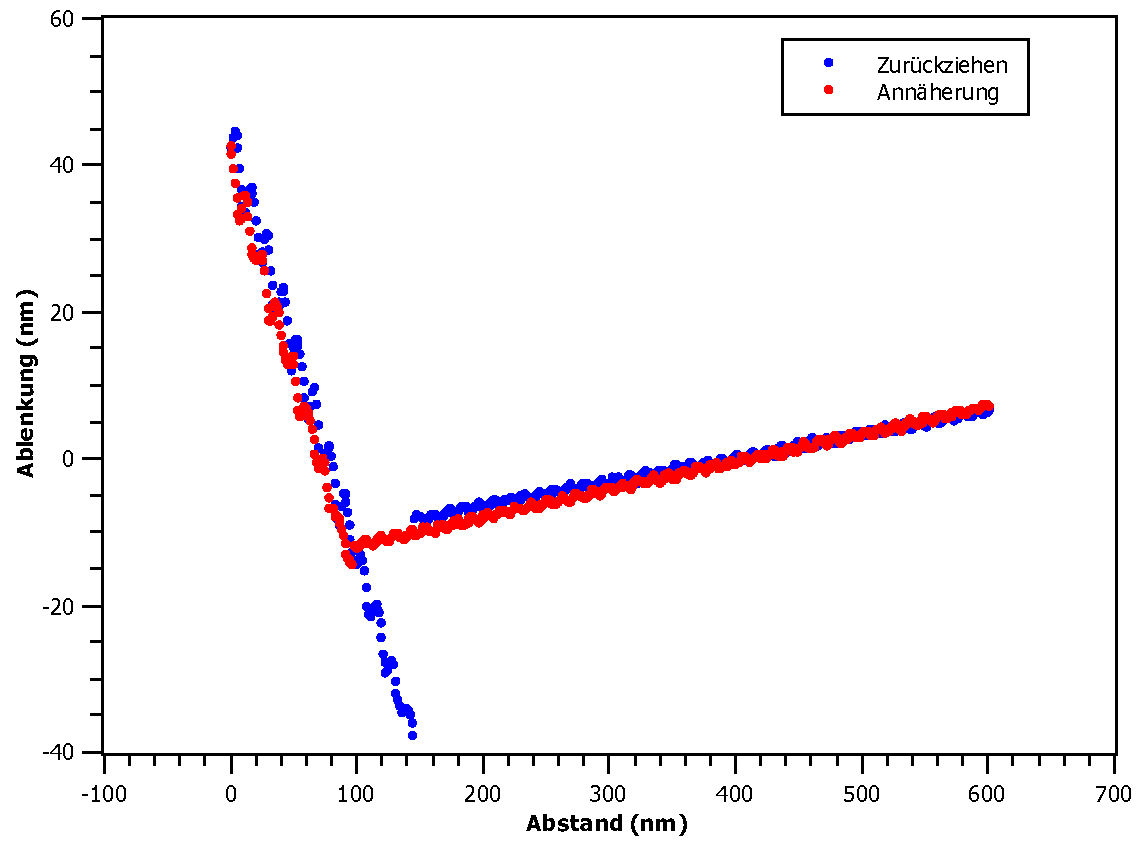
\includegraphics[width=.49\linewidth]{images/Kali/DS1}}
			\subcaptionbox{snap-off $s=\SI{35.1}{nm}$  \label{fig_kali_ds2}}{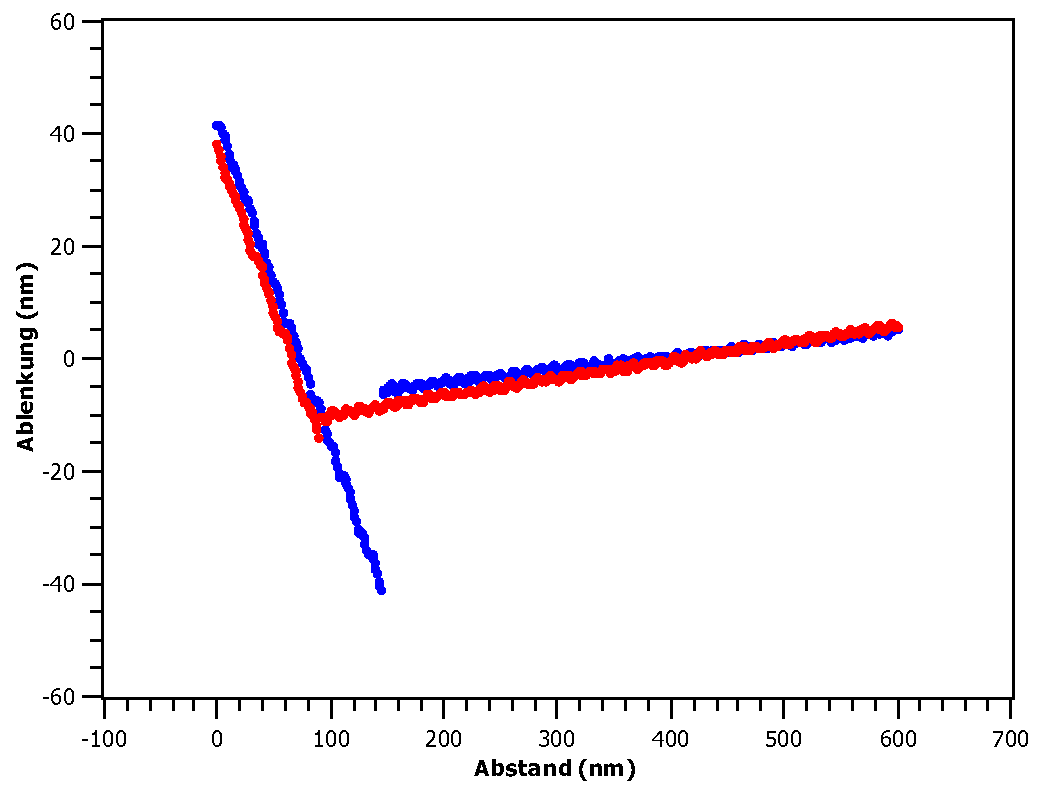
\includegraphics[width=.49\linewidth]{images/Kali/DS2}}
			\subcaptionbox{snap-off $s=\SI{25.6}{nm}$  \label{fig_kali_ds3}}{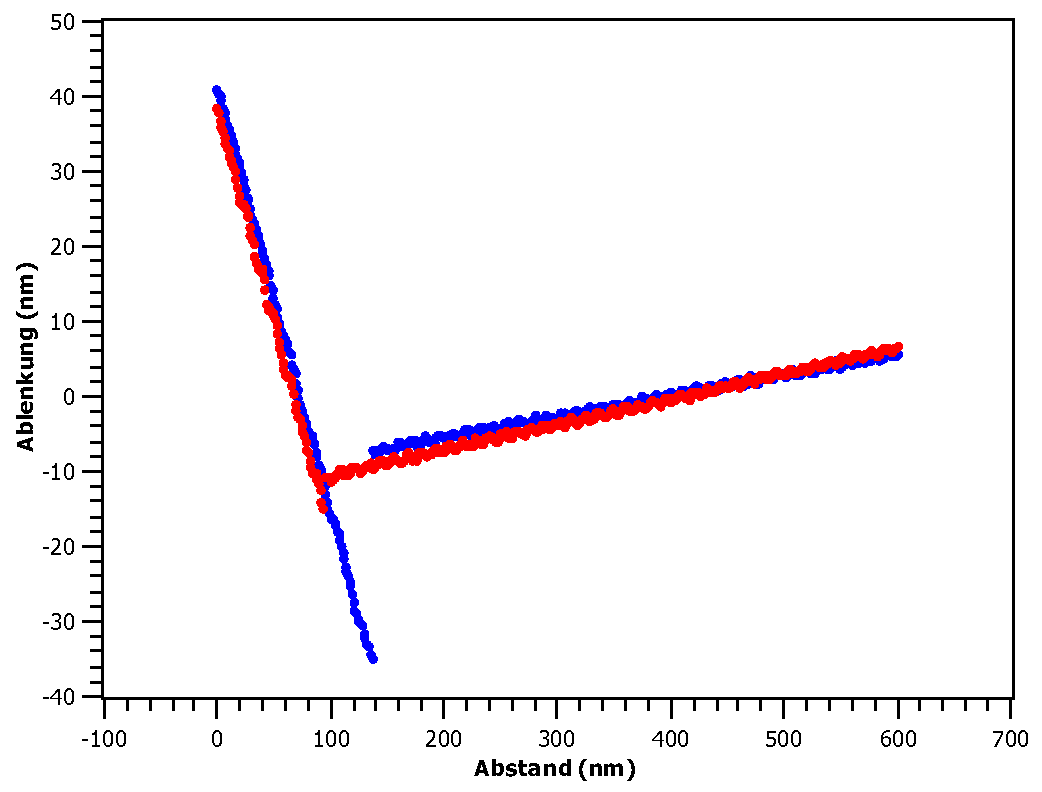
\includegraphics[width=.49\linewidth]{images/Kali/DS3}}
			\subcaptionbox{snap-off $s=\SI{26.3}{nm}$  \label{fig_kali_ds4}}{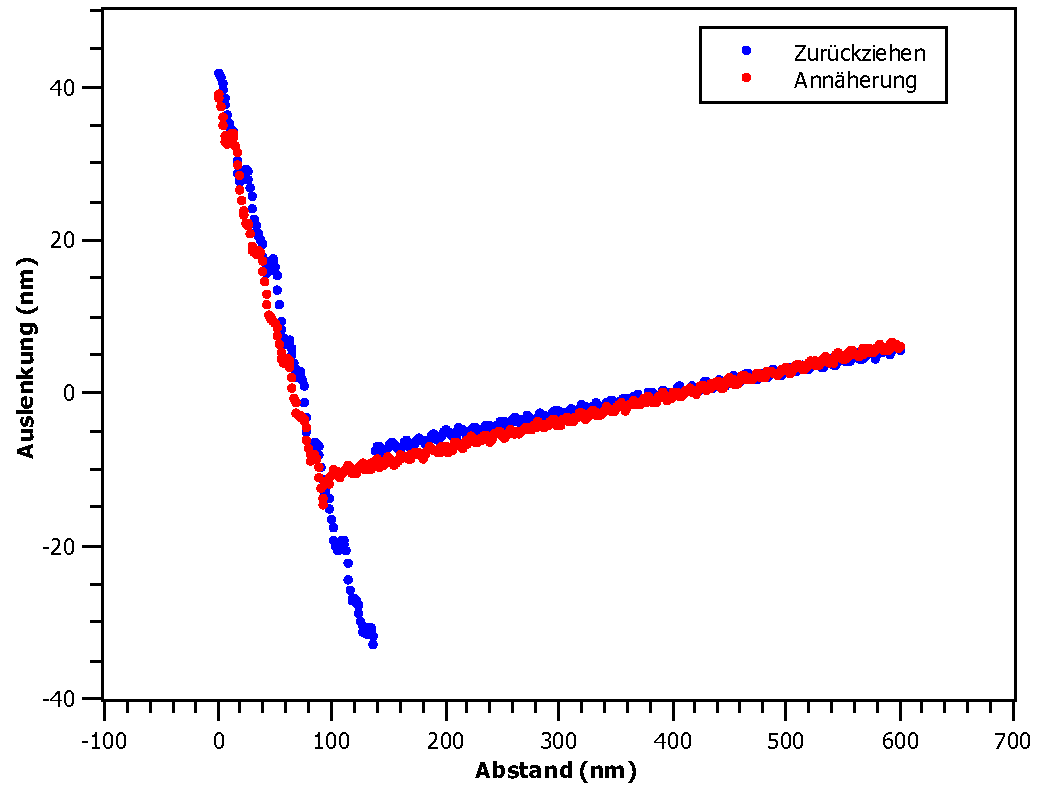
\includegraphics[width=.49\linewidth]{images/Kali/DS4}}
			\subcaptionbox{snap-off $s=\SI{28.0}{nm}$
			\label{fig_kali_ds5}}{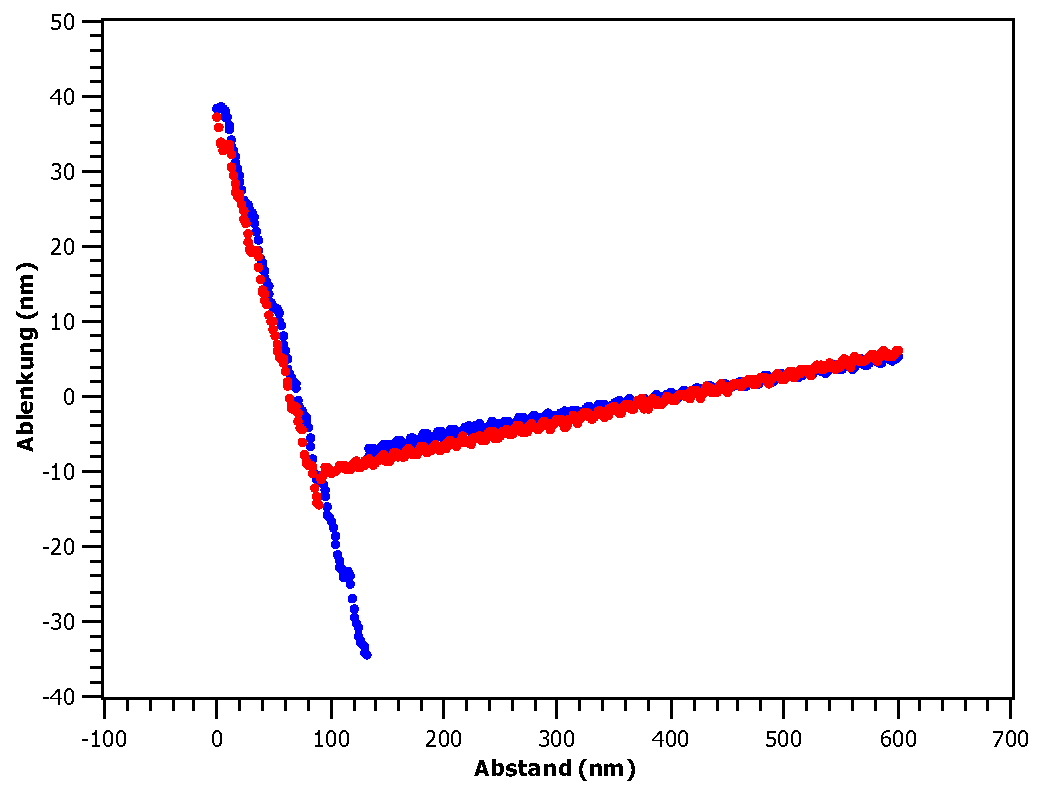
\includegraphics[width=.49\linewidth]{images/Kali/DS5}}
			\caption{Kraft-Abstands-Spektroskopie der Kalibrierprobe. Gemittelter snap-off $s=\SI{24.1}{nm}$.}
\end{figure}
\begin{figure}[H]
			\centering
			\subcaptionbox{snap-off $s=\SI{46.2}{nm}$  \label{fig_dvd_ds1}}{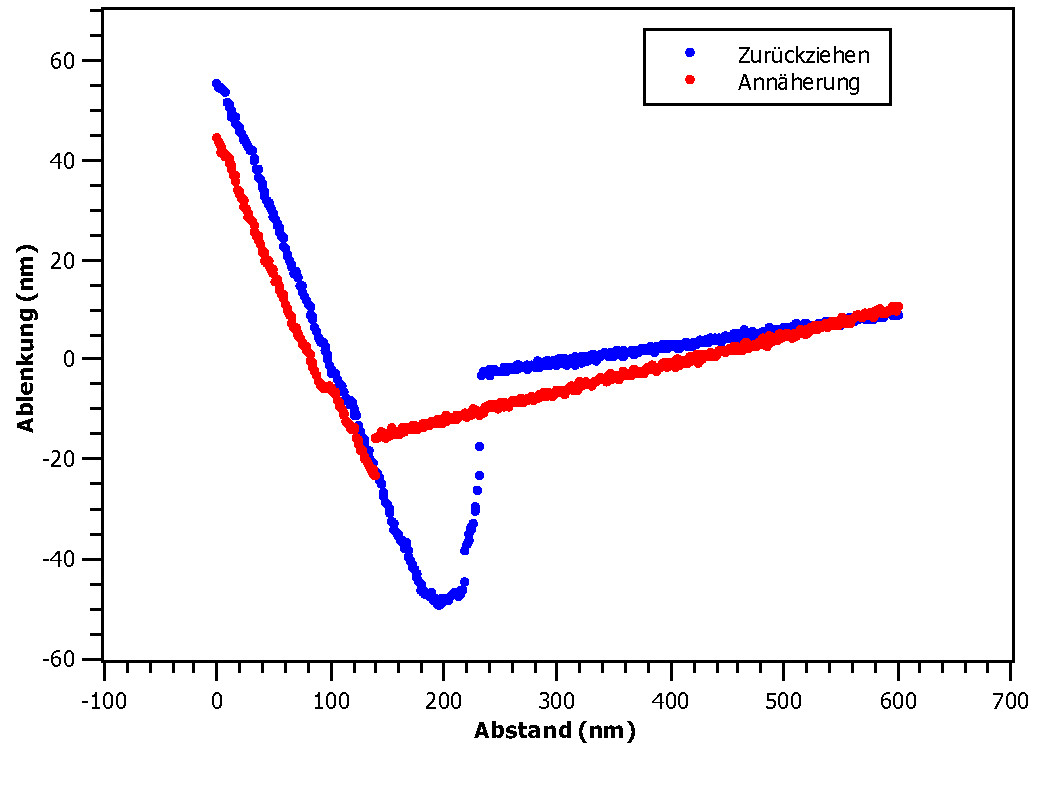
\includegraphics[width=.49\linewidth]{images/DVD/DS1}}
			\subcaptionbox{snap-off $s=\SI{50.0}{nm}$  \label{fig_dvd_ds2}}{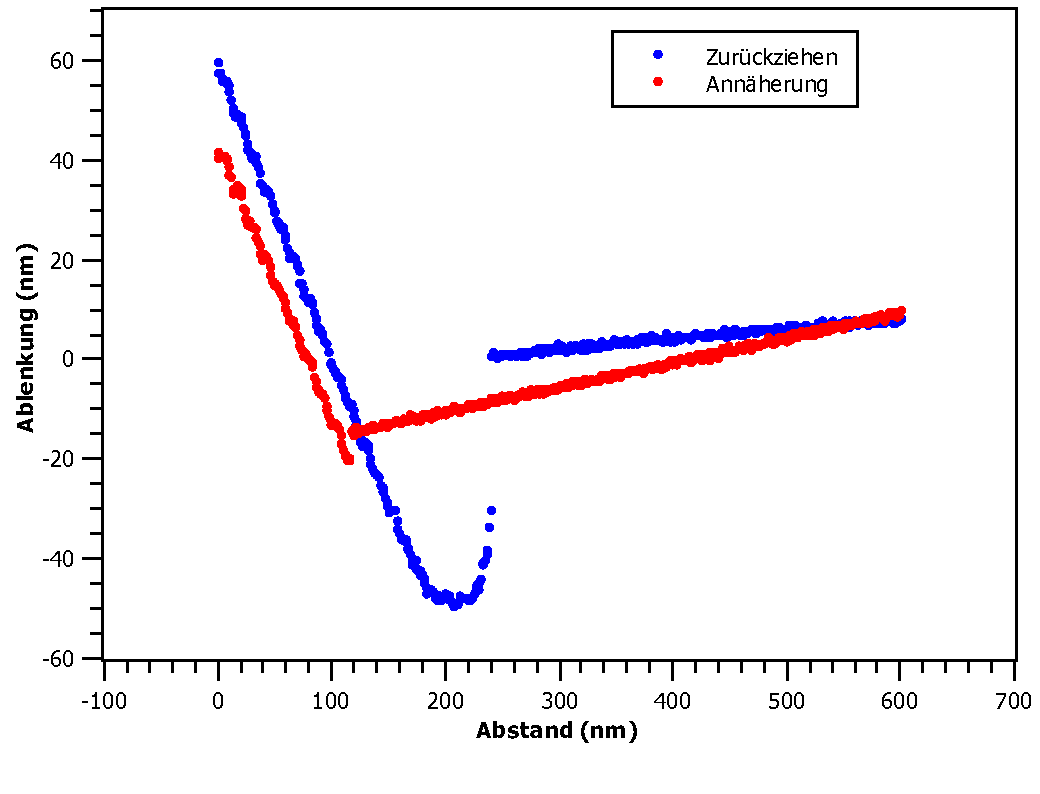
\includegraphics[width=.49\linewidth]{images/DVD/DS2}}
			\subcaptionbox{snap-off $s=\SI{42.4}{nm}$  \label{fig_dvd_ds3}}{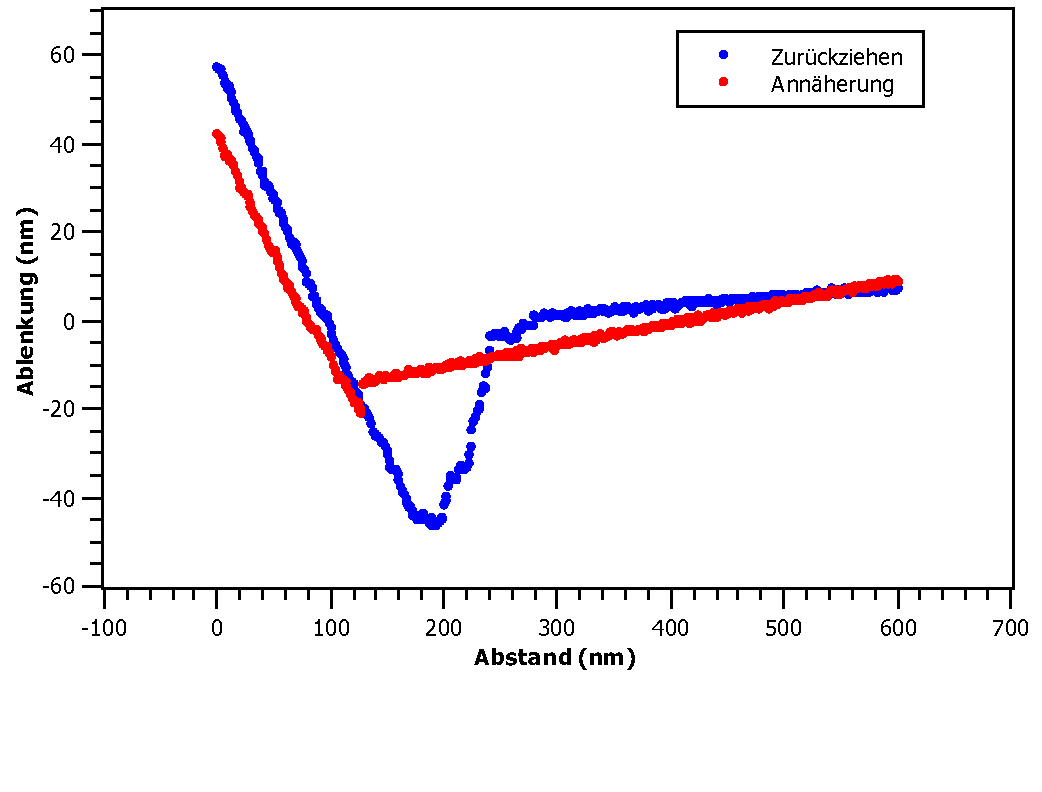
\includegraphics[width=.49\linewidth]{images/DVD/DS3}}
			\subcaptionbox{snap-off $s=\SI{44.2}{nm}$  \label{fig_dvd_ds4}}{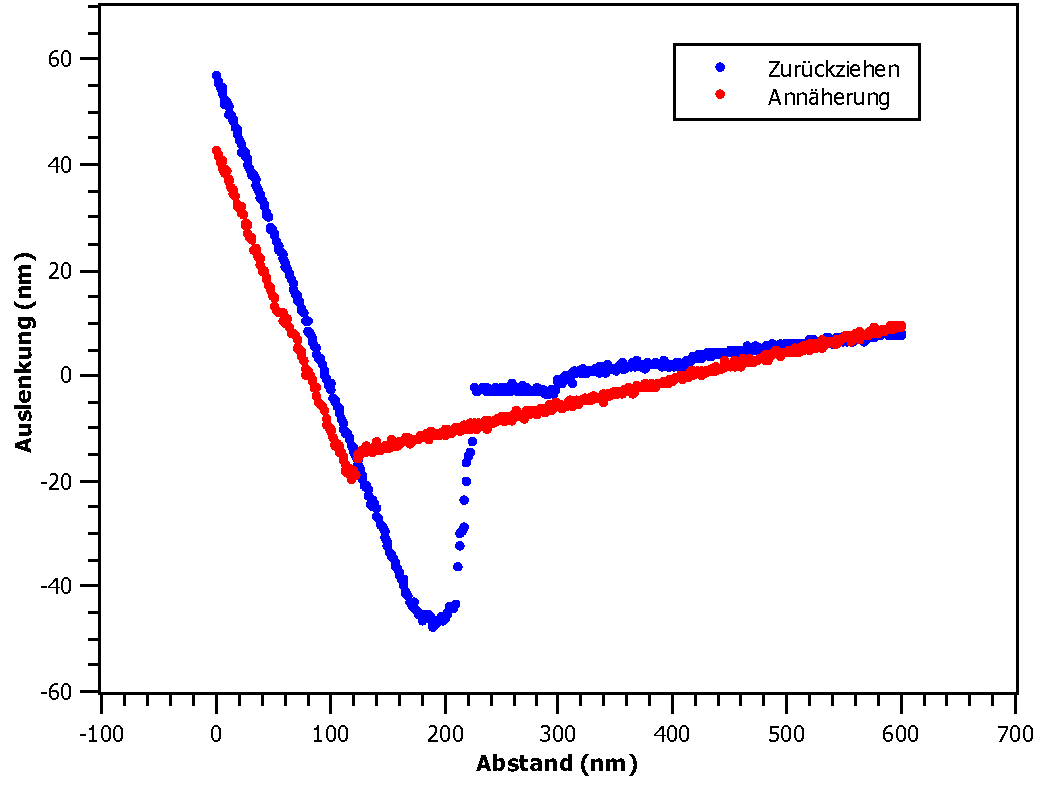
\includegraphics[width=.49\linewidth]{images/DVD/DS4}}
			\subcaptionbox{snap-off $s=\SI{39.8}{nm}$
			\label{fig_dvd_ds5}}{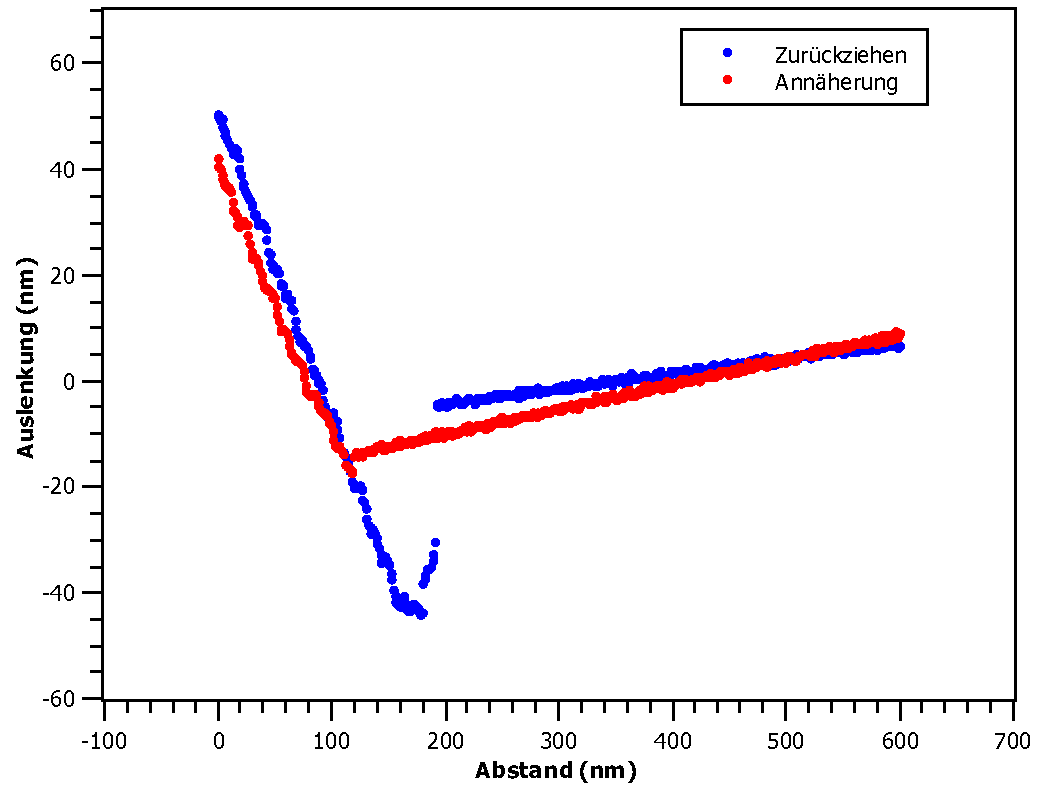
\includegraphics[width=.49\linewidth]{images/DVD/DS5}}
			\caption{Kraft-Abstands-Spektroskopie der Probe 1 auf einem der Maxima von \cref{fig_dvd_top}. Gemittelter snap-off $s=\SI{44.5}{nm}$.} % Pit oder Peak?
			\label{fig_dvd_ds}
\end{figure}
\begin{figure}[H]
			\centering
			\subcaptionbox{snap-off $s=\SI{46.2}{nm}$\label{fig_cd_ds1}}{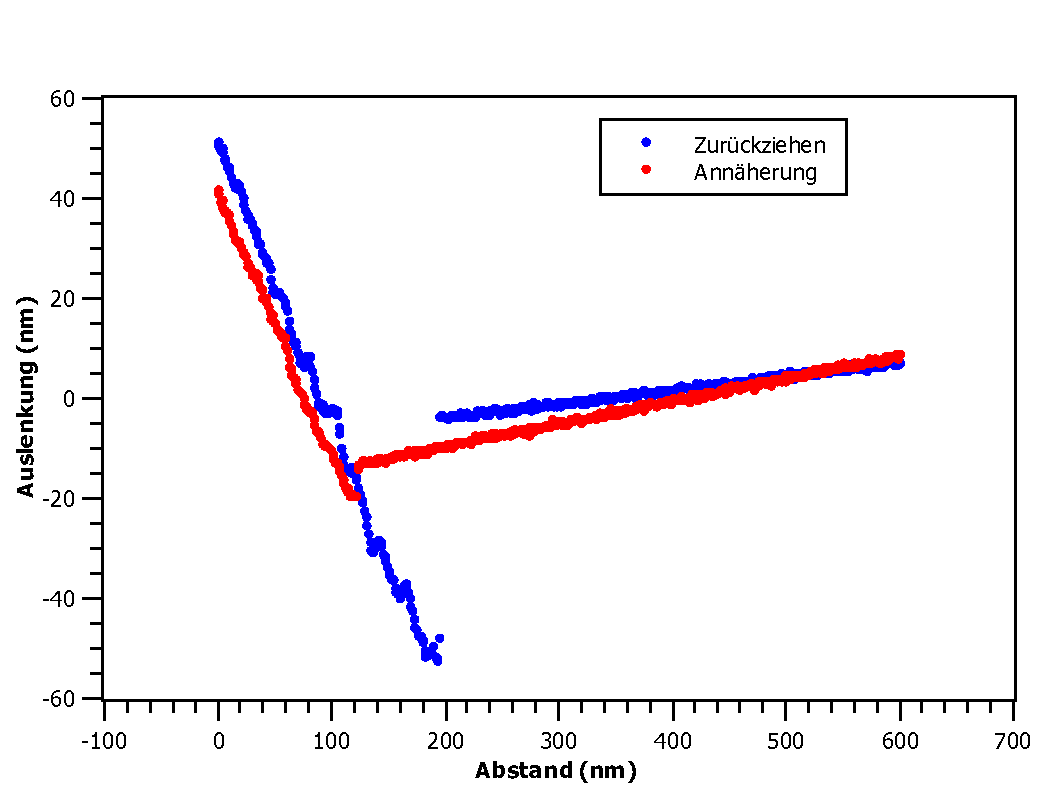
\includegraphics[width=.49\linewidth]{images/CD/DS1}}
			\subcaptionbox{snap-off $s=\SI{50.2}{nm}$\label{fig_cd_ds2}}{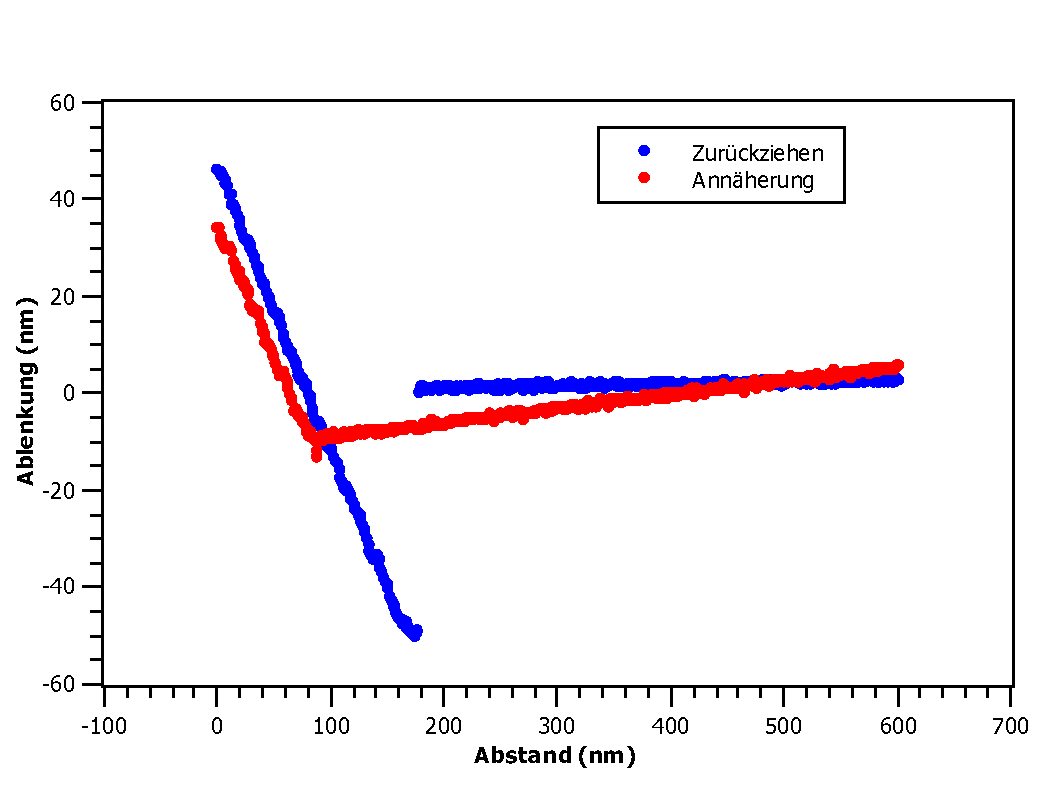
\includegraphics[width=.49\linewidth]{images/CD/DS2}}
			\subcaptionbox{snap-off $s=\SI{53.5}{nm}$\label{fig_cd_ds3}}{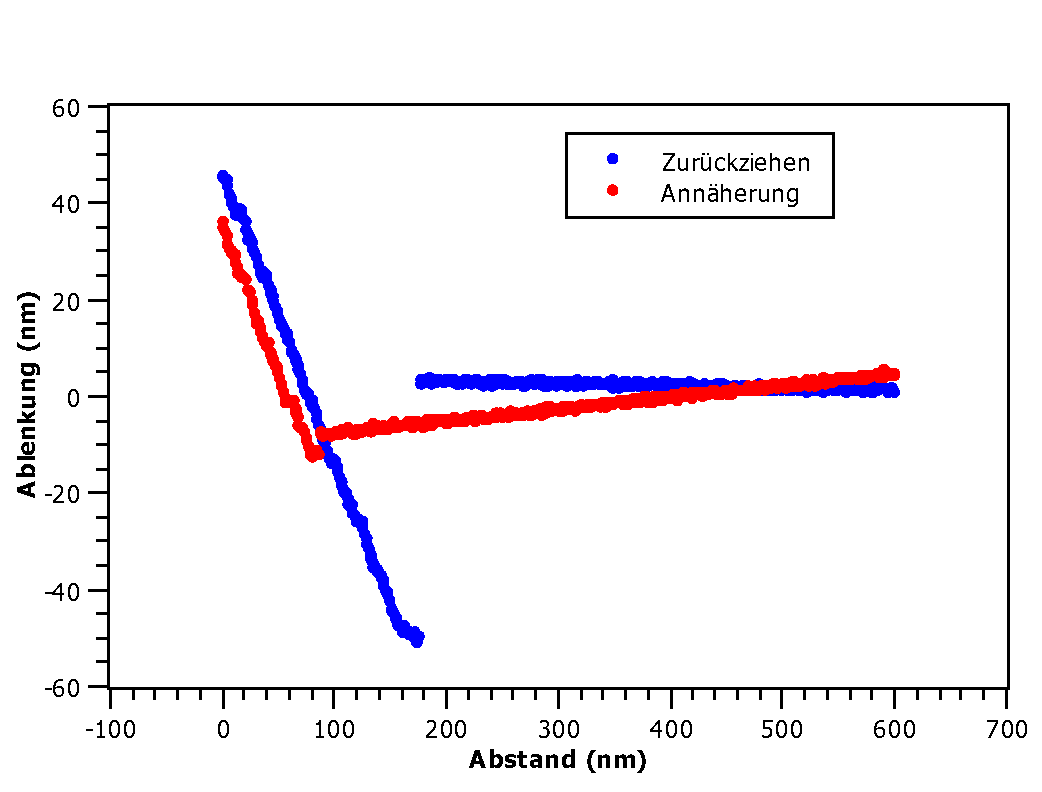
\includegraphics[width=.49\linewidth]{images/CD/DS3}}
			\subcaptionbox{snap-off $s=\SI{53.7}{nm}$\label{fig_cd_ds4}}{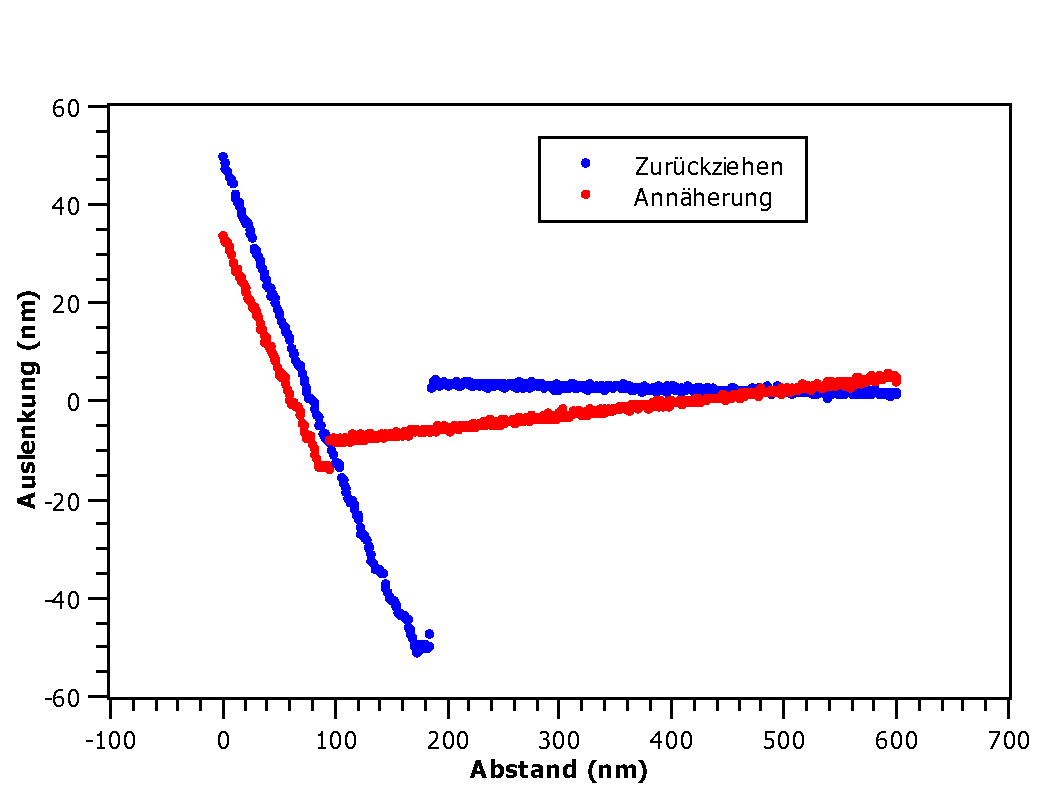
\includegraphics[width=.49\linewidth]{images/CD/DS4}}
			\subcaptionbox{snap-off $s=\SI{47.8}{nm}$
			\label{fig_cd_ds5}}{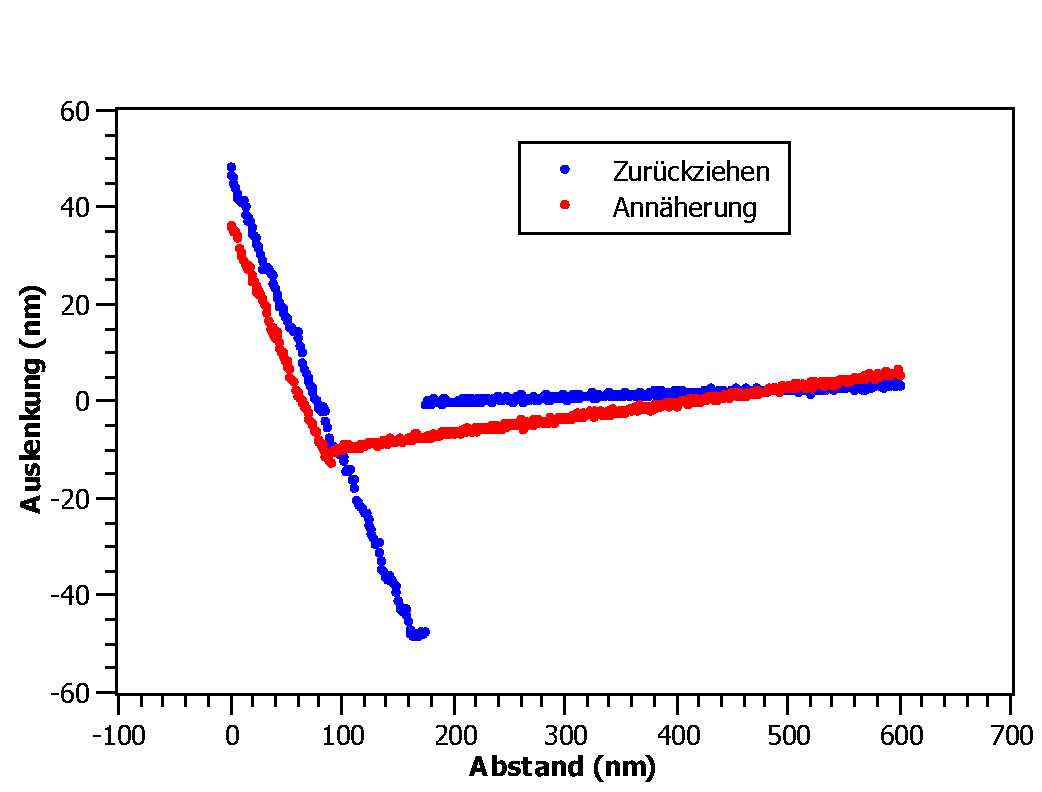
\includegraphics[width=.49\linewidth]{images/CD/DS5}}
			\caption{Kraft-Abstands-Spektroskopie der Probe 2 auf einem der Maxima von \cref{fig_cd_top}. Gemittelter snap-off $s=\SI{50.6}{nm}$.} % Pit oder Peak?
			\label{fig_cd_ds}
\end{figure}
\begin{figure}[H]
			\centering
			\subcaptionbox{snap-off $s=\SI{33.3}{nm}$\label{fig_br_ds1}}{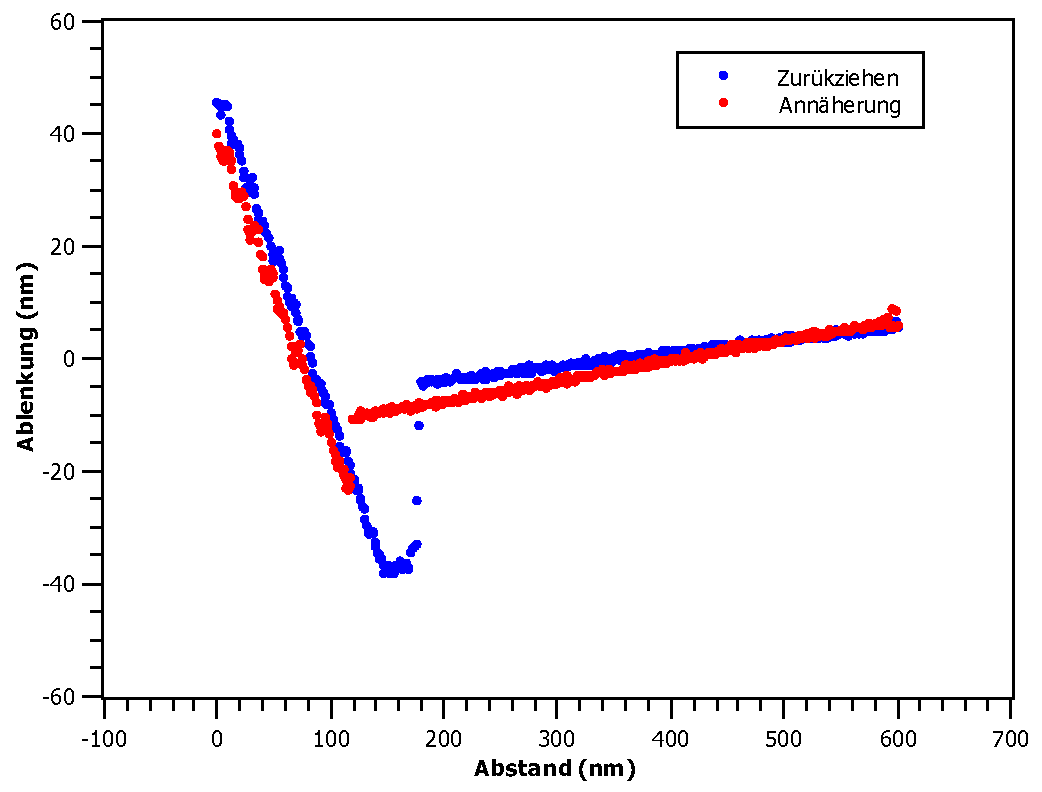
\includegraphics[width=.49\linewidth]{images/BR/DS1}}
			\subcaptionbox{snap-off $s=\SI{35.6}{nm}$\label{fig_br_ds2}}{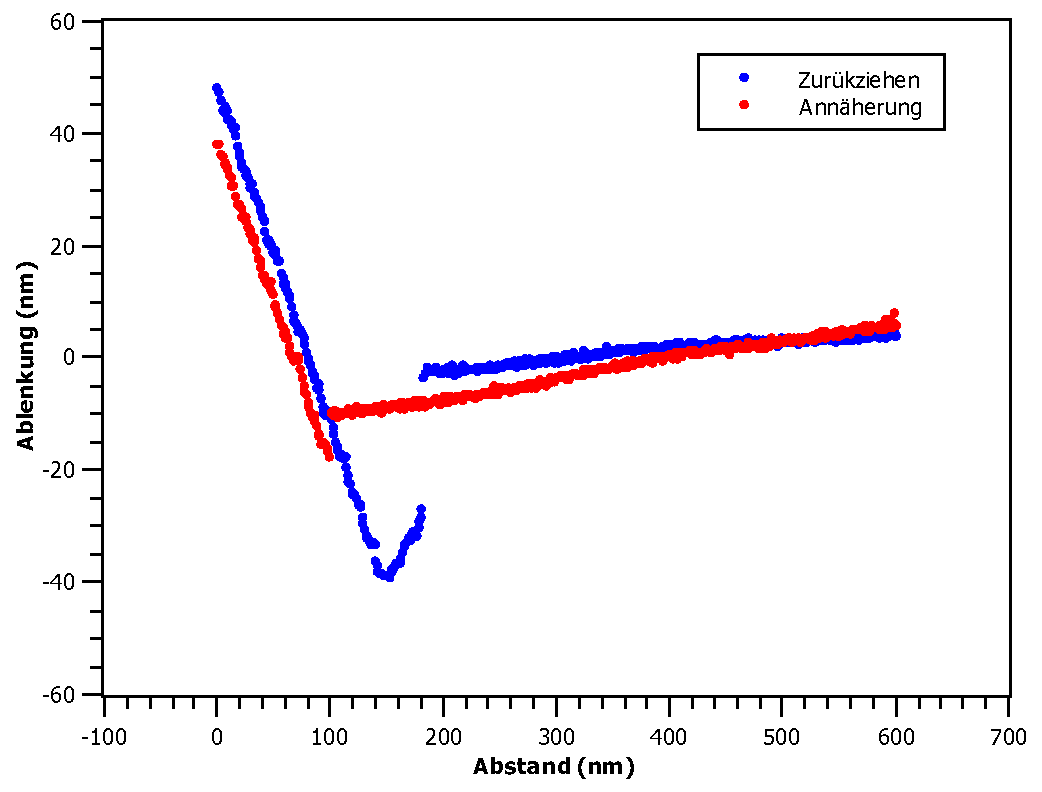
\includegraphics[width=.49\linewidth]{images/BR/DS2}}
			\subcaptionbox{snap-off $s=\SI{35.3}{nm}$\label{fig_br_ds3}}{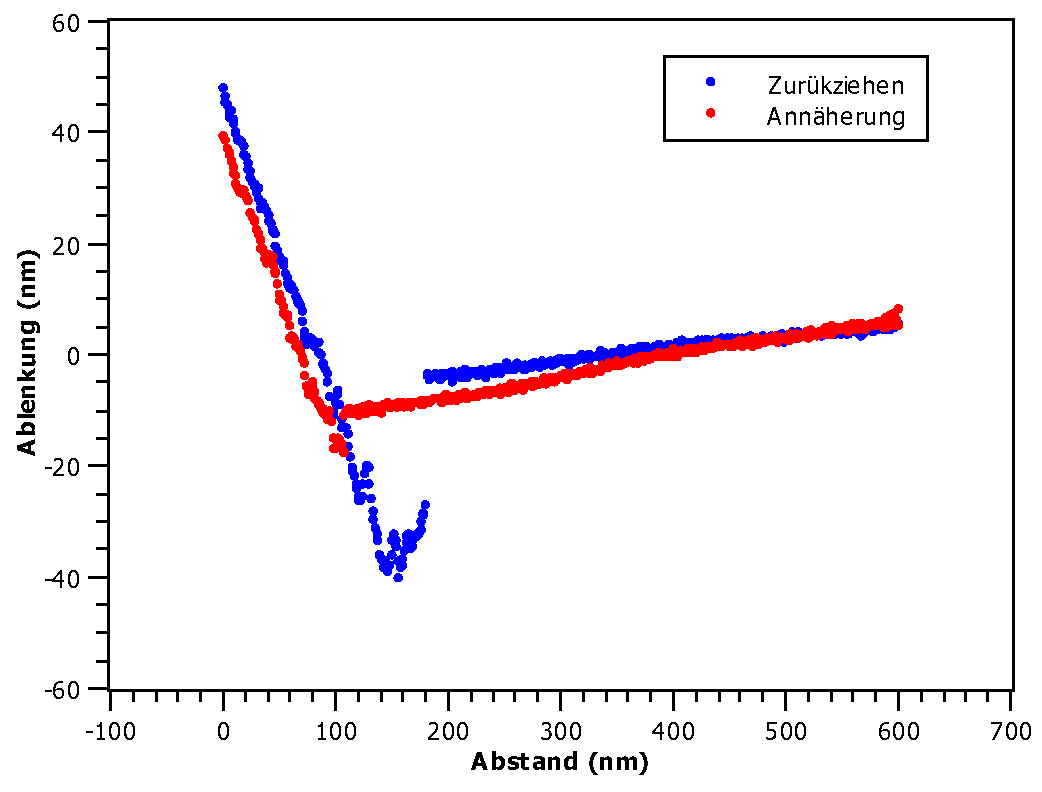
\includegraphics[width=.49\linewidth]{images/BR/DS3}}
			\subcaptionbox{snap-off $s=\SI{35.7}{nm}$\label{fig_br_ds4}}{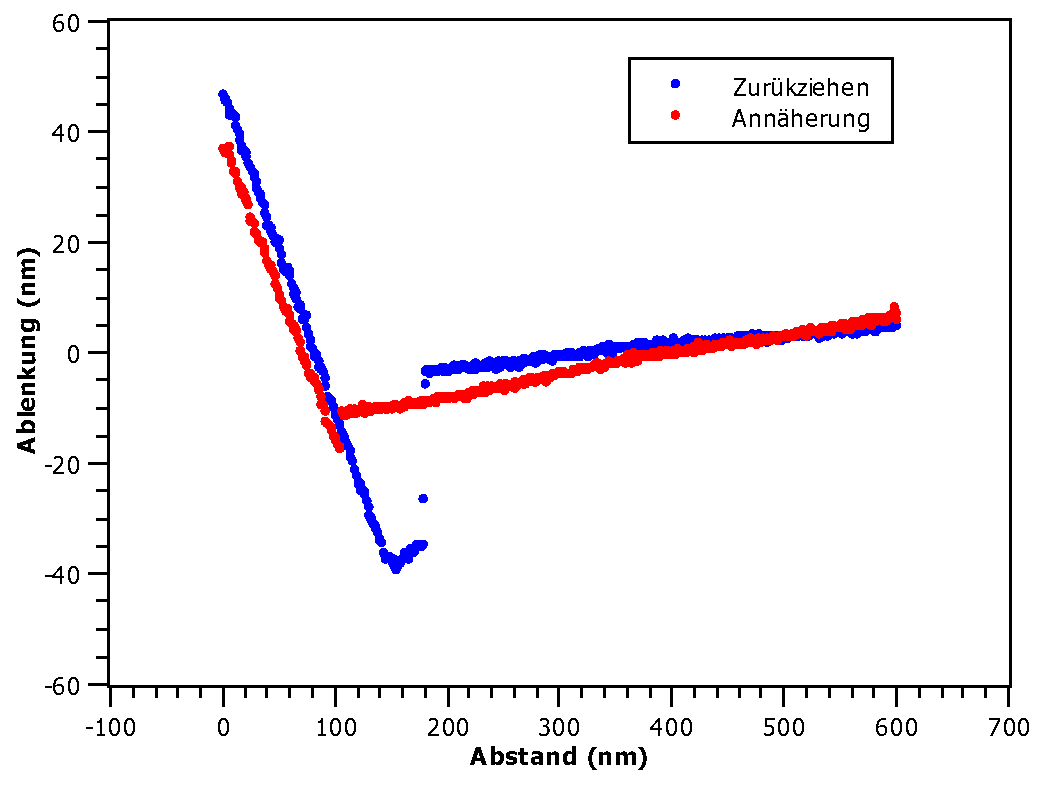
\includegraphics[width=.49\linewidth]{images/BR/DS4}}
			\subcaptionbox{snap-off $s=\SI{36.4}{nm}$
			\label{fig_br_ds5}}{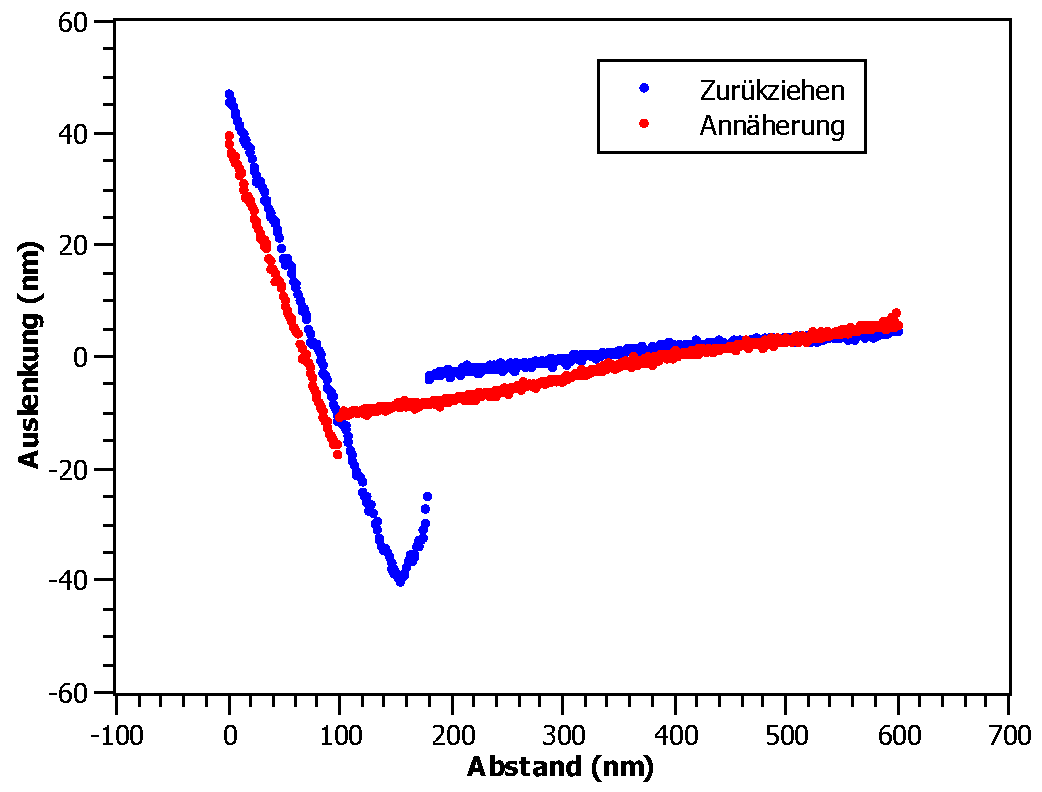
\includegraphics[width=.49\linewidth]{images/BR/DS5}}
			\caption{Kraft-Abstands-Spektroskopie der Probe 3 in einem der Minima von \cref{fig_br_top}. Gemittelter snap-off $s=\SI{35.3}{nm}$.} % Pit oder Peak?
			\label{fig_br_ds}
\end{figure}

%TODO Check Picture quality: Skalierung Achsen, Farben, Winkel etc
%TODO Fix new pages flow

\end{document}
